\documentclass[11pt,oneside]{uhthesis}
%\usepackage{subfigure}
\usepackage[linesnumbered,lined,titlenumbered,ruled]{algorithm2e}
\usepackage[flushleft]{threeparttable}
\usepackage{amsmath}
\usepackage{amssymb}
\usepackage{amsbsy}
\usepackage{mathpazo}
\usepackage{float}
\usepackage{braket}
\usepackage{subcaption}
\usepackage{graphicx}

%\floatstyle{ruled}
%\restylefloat{table}

\renewcommand{\tablename}{Tabla}
%\dontprintsemicolon

\renewcommand{\vec}[1]{\boldsymbol{#1}}
\newcommand{\diff}[1]{\ensuremath{\mathrm{d}#1}}

\DeclareMathOperator*{\argmax}{\arg\! max}
\DeclareMathOperator*{\argmin}{\arg\! min}

\title{Algoritmo de clustering y trayectorias aplicados al análisis de la segregación poblacional} 
\author{Manuel Santiago Férnandez Arias}
\advisor{MsC. Dafne García de Armas}
\degree{Licenciado en Ciencia de la Computación}
\faculty{Facultad de Matemática y Computación}
\date{}
\logo{Graphics/uhlogo}
\makenomenclature

\renewcommand{\vec}[1]{\boldsymbol{#1}}
%\newcommand{\diff}[1]{\ensuremath{\mathrm{d}#1}}

\begin{document}

%\frontmatter
\maketitle

%\include{FrontMatter/Dedication}
%===================================================================================
% Chapter: Agradecimientos
%===================================================================================
\chapter*{Agradecimientos}\label{chapter:thanks}
\addcontentsline{toc}{chapter}{Agradecimientos}
%===================================================================================
%===================================================================================
% Chapter: Opinión del Tutor
%===================================================================================
\chapter*{Opinión del Tutor}\label{chapter:supervisor_opinion}
\addcontentsline{toc}{chapter}{Opinión del Tutor}
%===================================================================================
%===================================================================================
% Chapter: Resumen
%===================================================================================
\chapter*{Resumen}\label{chapter:abstract}
\addcontentsline{toc}{chapter}{Resumen}
%===================================================================================
\include{FrontMatter/Contents}

\mainmatter
	
%===================================================================================
% Chapter: Introducción
%===================================================================================
\chapter*{Introducción}\label{chapter:introduction}
\addcontentsline{toc}{chapter}{Introducción}

La segregación residencial es un concepto que nos acompaña desde la década del 20 en el pasado siglo. En los últimos años los estudios sobre las condiciones de vida, las desigualdades, la diferenciación socio-espacial, la vulnerabilidad, la pobreza y las brechas sociales, han alcanzado una gran importancia en diversas disciplinas principalmente en las ciencias sociales. La compresión de dicho fenómeno tiene un gran significado para las instituciones públicas y gubernamentales. Las mismas, respaldadas en estos análisis, tienen oportunidad de mejorar las políticas y condiciones impulsando un acceso más justo e igualitario a los servicios e infraestructuras en cada localidad.

En la literatura existen dos definiciones fundamentales para la segregación residencial. La visión jerárquica \cite{Ortega2018LaSR}, definida por el proceso donde los grupos étnicos de mayor poder condicionan las oportunidades de acceso al suelo urbano a aquellos grupos de menos poder. Por otra parte, el enfoque geográfico \cite{Merkel2014QueEY}, en el que estará basado este estudio, está caracterizado por las relaciones espaciales, donde se afirma que cualquier grupo desigualmente distribuido en un espacio presenta segregación.

Las marcadas diferencias sociales determinan la composición de los vecindarios y afectan en gran medida muchos aspectos de la vida urbana: el acceso a educación, a la salud y a los servicios en general. Aquí radica la necesidad de los estudios de segregación que permitan encontrar vulnerabilidades en las ciudades con el fin de erradicarlas o mejorar los indicadores. 

En la literatura se reportan numerosos estudios sobre la segregación residencial en todas las ciencias sociales, principalmente en la sociología. Analizar dicho fenómeno no es una tarea sencilla pero debido al notable crecimiento de la ciencia de datos, análisis estadísticos de grandes volúmenes de información y el aprendizaje por computadora han provocado que estas tecnologías se viertan también en el estudio de segregación. Existen diferentes metodologías y métodos a la hora de abordar el problema en cuestión. Uno de las técnicas más novedosas es el uso de algoritmos de clustering \cite{Morissette2013TheKC}. La presente investigación se centra en el desarrollo de un algoritmo que permita detectar segregación residencial empleando los algoritmos de clustering y las Trayectorias Simples Modificadas \cite{RandonFurling2018FromUS}. Una trayectoria constituye una curva que recorre todo un territorio divido en pequeñas estructuras partiendo de un punto inicial. Normalmente en la literatura se hace referencia a las estructuras en la que queda dividida un territorio con el nombre de bloques censales. Las trayectorias simples son aquellas donde en cada bloque censal de la trayectoria se almacena una proporción entre la variable de estudio y la población total en dicho bloque.\\\\


Por lo anteriormente expuesto, se establecen los siguientes objetivos:


\subsection*{Objetivo general:}
Detectar la existencia de segregación mediante una propuesta de solución basada en algoritmos de clustering.
\subsection*{Objetivos específicos:}
\begin{itemize}
	
	\item Estudiar el estado del arte de los métodos de trayectorias y algoritmos de clustering utilizados en investigaciones sobre la segregación residencial.
	
	\item Definir métricas de comparación para evaluar la factibilidad de emplear dichos algoritmos en la detección de diferentes tipos de segregación residencial.
	

	
\end{itemize}



Este trabajo estará divido en 3 capítulos. En el capítulo 1 se resumen los principales resultados en materia de segregación y se discuten los algoritmos de clustering empleados en este tipo de problemas. En el capítulo 2 se formaliza el problema central que se aborda en este trabajo, se propone una estrategia para analizar la \textbf{segregación poblacional} y se formula una medida para su validación. En el capítulo 3 se describen los experimentos realizados. Finalmente aparecen las conclusiones, recomendaciones y la bibliografía consultada.

%\subsection*{Contribuciones}

%\subsection*{Organización de la Tesis}

%===================================================================================
%===================================================================================
% Chapter: Estado del Arte
%===================================================================================

\chapter{Estado del Arte}
Guerras, incendios forestales, caídas de la bolsa, ataques informáticos, crisis alimentaria, conflictos bélicos, calentamiento global, por solo citar alguno de los problemas que nos atacan en la actualidad. Cada día es más difícil analizar las consecuencias de lo local sin mirar al mundo exterior. En un mundo cada vez más globalizado y a su vez separado en diferentes sectores, clases sociales, religiones u orientaciones políticas; se hace necesario un análisis profundo de la realidad contemporánea para sacar conclusiones objetivas acerca de la cotidianidad, así como, intentar fomentar la toma de decisiones en gobiernos y grandes transnacionales para suavizar o en el mejor de los casos, erradicar ciertas diferencias entre los distintos sectores de la sociedad.

Si existe algo increíble en el mundo que vivimos hoy, es que si bien, somos una sociedad completamente globalizada cada vez vivimos más dispersos en grupos aislados. La globalización esta propiciada en una parte por las increíbles transformaciones en el campo de la informática, las telecomunicaciones y el comercio, unido a la innegable presencia de las potencias mundiales detrás del modelo de pensamiento y la forma de concebir el mundo. ¿Cómo es posible entonces que se explique la existencia de la segregación residencial?

\section{Orígenes de la segregación}

Para poder comenzar un estudio objetivo sobre la segregación residencial se hace necesario resaltar la siguiente pregunta: ¿Qué se entiende por segregación residencial y social? Dicho en términos de White (1983), la segregación en sentido geográfico consiste en la desigual distribución de los grupos sociales en el espacio físico \cite{Rodrguez2008SegregacinRS}. 

Resulta conveniente analizar la existencia de conceptos que refieren a aspectos de ciertos problemas sociales que no son fácilmente separables. Tal es el caso de los conceptos de: “segregación territorial”, “segregación residencial” y “segregación social”. Muchas veces estos conceptos resultan intercambiables. El último de ellos, en disímiles ocasiones se expresa a través de los dos anteriores, sin embargo, no puede ser explicado íntegramente por ellos. “Segregación social”, es un concepto mucho más complejo, y su análisis está marcado por otras variables de lo social que no guardan relación necesaria con el territorio, como pueden ser la situación respecto al mercado de empleo, al acceso a la educación y a los servicios en general. Usualmente hace referencia a las diferencias culturales, normativas, simbólicas y de sensibilidad entre los individuos. “En una sociedad de castas, por ejemplo, la segregación social es virtualmente absoluta, con independencia de la forma en que estas castas se localizan en el territorio; así, en ese caso extremo, la eventual cercanía física de las castas no promovería la interacción entre ellas” \cite{Merkel2014QueEY}.

En la década de los años 20 del pasado siglo, varias disciplinas en el campo de las ciencias sociales mostraron interés por el análisis de los patrones de segregación espacial en las ciudades. La ciudad estadunidense de Chicago fue uno de los epicentros del creciente auge sobre el estudio de dicha problemática. Basándose en analogías de la ecología y la botánica Robert Park presento una representación del mosaico urbano en 1915 \cite{Goist1971CityA}, que tuvo vital importancia en los años venideros. En 1925 E.W. Burgess  presentó un diseño predominantemente concéntrico \cite{Park1984TheCS}. El modelo clásico como luego se conocería la representación de Burgess, describía como los pobres vivían en el centro de la ciudad y los que estaban en mejores condiciones económicas ocupaban los anillos de creciente status social a medida que se alejaban del centro.

\begin{figure}[h!]
	\centering
	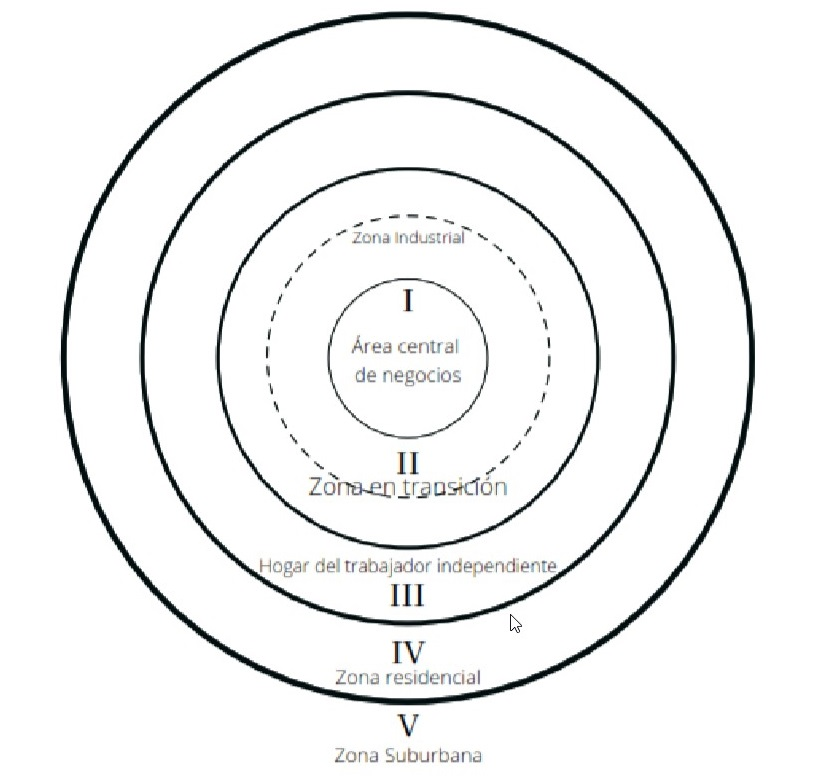
\includegraphics[width=8cm, height=8cm]{Images/Modelo.jpg} 
	\caption{Modelo de Burgues}
\end{figure} 

El modelo clásico se convirtió en un punto de partida para los estudios de segregación, muchas personalidades de la época afines al tema realizaron aportes y contribuciones sobre el mismo. Por un lado, se encontraban las personalidades cuyos ejes de investigación se centraba en los alineamientos topográficos y rutas de comunicación, como fue el caso del sociólogo Homer Hoyt en 1939 \cite{Adams2005HoytH1} y en el otro extremo quienes centraban su atención en el rol de ciertos hitos culturales e históricos como los puntos de anclaje para la élite en los centros de algunas ciudades, como fue: Walter Firey en la ciudad de Boston \cite{Gilmore1947LandUI}.	

A pesar del auge de los estudios de segregación, pareciera que después de abrir el camino hacia el análisis residencial espacial, los sociólogos hubieran perdido su interés en esta cuestión para volver a su tema tradicional orientado a entender el comportamiento de las instituciones sociales y la naturaleza del cambio    social, especialmente como resultado de la urbanización y del impacto del urbanismo como forma   de vida \cite{Manella2014LouisW}. Esto provocó una escasez en cuanto a las publicaciones referentes al tema durante casi una década.
A finales de 1940 se retomaron los estudios enfocados a la medición de la segregación. Uno de los índices que resaltó en estos estudios, sin dudas el más conocido, fue el índice de disimilitud de Duncan \cite{Duncan1955AMA}. El índice de disimilitud representa la proporción del grupo minoritario de una población que tendría que cambiar de residencia para obtener una distribución igualitaria en toda la ciudad. Otros índices surgieron en el transcurso de ese período, pero compartían la limitante de que solo median la segregación en cuanto a dos grupos, lo que refleja el marcado conflicto racial de la época entre personas blancas y negras \cite{Feitosa2004SpatialMO}.
A comienzos de la década de los sesenta se publicó el que para muchos es considerado el libro más influente de la planificación urbana \cite{Jacobs1961TheDA} \cite{NT}. Jane Jacobs, autor del libro, estableció precedentes importantes para el movimiento del Nuevo Urbanismo con respecto a combatir la segregación. Por un lado, defendía la conservación de las diferencias naturales dentro de la ciudad, pero se manifestó en contra de las zonas monopropósito, impulsando en gran medida el desarrollo de las zonas multipropósito que mezclaban trabajo, comercio y residencia. Impulsado principalmente por el modelo desarrollado por Alonso en 1964 \cite{Kirwan1966BookRL}, basado en patrones económico-espaciales para las ciudades, dicha temática pasó a ser de gran interés para los geógrafos. 

\begin{figure}[htb]
	\centering
	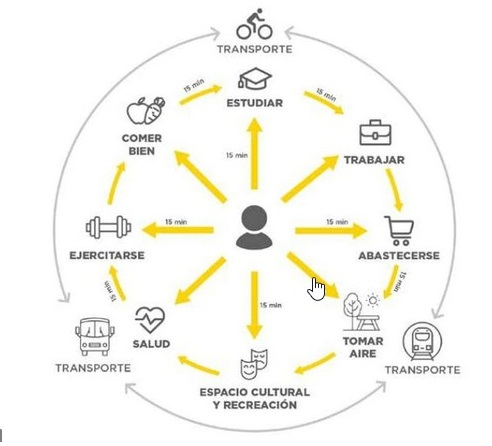
\includegraphics[width=8cm, height=8cm]{Images/ZonaMultiproposito.jpg} 
	\caption{Zonas Multipropósitos}
\end{figure} 

Para finales de los 60 y principio de los 70 los notables avances de las ciencias de la computación, representaron un punto de inflexión en el estudio de la segregación residencial. Los geógrafos contaban con una mayor capacidad para generar “ecologías factoriales” de las ciudades \cite{Clarke1966PopulationPI} \cite{Johnston1978BerryBJ}. Los mapas generados produjeron descripciones bastante matizadas y desagregadas de patrones de distribución espacial de los distintos grupos sociales en las ciudades. Se basaban en correlaciones de análisis factorial de clústeres de variables que parecían estar fuertemente relacionadas.

\begin{figure}[htb]
	\centering
	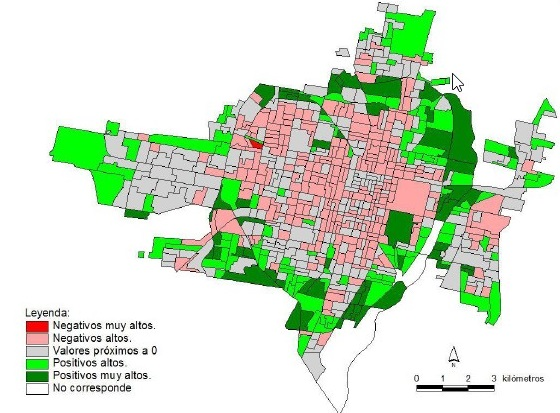
\includegraphics[width=8cm, height=7cm]{Images/EcologiaFactorial.jpg} 
	\caption{Ecología Factorial}
\end{figure} 

Estos clústeres incluían varias características: raza, status socio-económico, edad, por solo citar las más comunes. En efecto estas agrupaciones apuntaban a comprender los procesos subyacentes \cite{Ward1975BrianTR} \cite{Downs1977MapsIM}, pero no lograban explicar realmente por qué la gente elegía determinado lugar para vivir, ni de qué manera se construían sus aspiraciones. En el año 1971 se publicó un artículo pionero en los modelos dinámicos de segregación, el cual si bien en sus inicios estuvo enfocado en el ámbito racial ha tenido una gran trascendencia en todos los estudios de segregación \cite{GoffetteNagot2010IntroducingLC}. Schelling, autor del artículo, propuso un modelo espacial basado en agentes, los cuales cambian su posición acorde a una función de “satisfacción”. Varios son los autores que se basaron en este artículo para trabajos posteriores demostrando la robustez de dicho modelo \cite{Ostolaza2001SobreMD} \cite{Banos2012NetworkEI}. Para finales de los 80, Douglas Massey y Nancy Denton, presentaron un artículo en el cual propusieron cinco dimensiones de segregación: uniformidad, exposición, concentración, centralización y agrupamiento, que pueden ser medidas cuantitativamente a través de índices de segregación \cite{Massey1988TheDO}. Este aporte tuvo gran impacto en los estudios de segregación pues por aquel entonces existía un extenso debate sobre cómo medir correctamente la segregación.

Para los años 2000 los temas vinculados al estudio de la segregación residencial socioeconómica han tenido una presencia constante en los debates académicos y en las agendas públicas de la mayoría de los países del mundo \cite{Luco2003SegregacinRE} \cite{Ham2021}. El basto número de investigaciones referentes a la segregación residencial del pasado siglo y del comienzo de este siglo nos permite afirmar que no es un problema asociado a la sociedad contemporánea, aunque en la actualidad dicha problemática se presenta con mayor visibilidad. Esto se debe a dos fenómenos fundamentales: un primer fenómeno está dado por los estudios recientes que sugieren la existencia un patrón segmentado de localización de los diferentes grupos socioeconómicos en las metrópolis regionales. Un segundo fenómeno es que el mero efecto estadístico, de los asuntos urbanos y metropolitanos han ganado preeminencia entre los problemas de base territorial. Sin embargo, la principal razón por la cual la segregación residencial es un punto más que necesario en la mayoría de las agendas de los debates académicos actuales sobre la sociedad en el mundo, es por las adversidades que la misma trae consigo. 

La visión negativa de la segregación residencial socioeconómica es producto del balance entre facetas contradictorias de la segmentación socioeconómica del espacio. Por una parte, están las desventajas para quienes experimentan dicha segmentación como una forma explícita o disimulada de exclusión y por otra, está el hecho de que para algunos grupos es una opción racional guiada por principios como la maximización de utilidad, la exclusividad, la distinción, la afinidad, la acumulación de activos, la construcción de redes o el acceso a recursos.


\section{Enfoques de los estudios de la segregación} 

La segregación residencial como problema social ha sido altamente estudiada. Siendo abordada por varias disciplinas como son: la sociología, la geografía, la historia y la economía, por solo nombrar las más relevantes. Sin embargo, vale destacar que dependiendo de la región y la época del estudio en cuestión los temas de investigación varían bastante. 

En los Estados Unidos se originaron los primeros estudios sobre dicha temática. Al comienzo los análisis se centraron en las diferencias de étnicas y raciales \cite{Feitosa2004SpatialMO}. Esta problemática, conocida y estudiada desde las primeras décadas del siglo pasado, se mantiene vigente hoy en día y siguen los estudios al respecto. En 2006, se realizó un estudio empleando el índice general de disimilitud, sobre varias ciudades de Estados Unidos. El mismo demostró que la raza continúa siendo un factor importante de segregación, haciendo énfasis en la calidad de educación y viviendas \cite{Selmi2005RaceIT}. El centro para servicio público Weldon Cooper de la Universidad de Virginia elaboró un mapa donde se puede ver la distribución geográfica de los distintos grupos raciales en Estados Unidos, a partir de los datos del censo de 2010 \cite{SDC}. El mapa ofrece una visualización de la distribución geográfica, densidad de población y diversidad racial de la población estadounidense en cada vecindario de todo el país y sirve de base para disímiles estudios acerca de la segregación racial en Estados Unidos \cite{WC}.

\begin{figure}[htb]
	\centering
	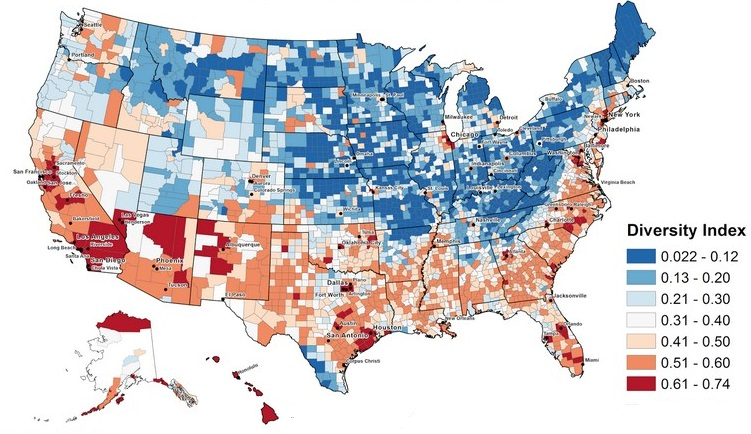
\includegraphics[width=8cm, height=5cm]{Images/WeldomCooper.jpg} 
	\caption{Mapa elaborado por la universidad de Weldon Cooper }
\end{figure} 

Sin embargo, vale destacar que la motivación principal de los estudios acerca de la segregación en los 
Estados Unidos de hoy está asociada a describir otro fenómeno: el claro crecimiento que ha tenido el empleo 
en el área suburbana con respecto al centro de la ciudad. Este creciente desplazamiento de la sociedad americana hacia las zonas no residenciales, resalta la necesidad de estudios de segregación sobre la misma, 
que en palabras de Park y Kwan: “se sabe muy poco sobre la segregación que viven las personas en contextos no 
residenciales“. Un estudio realizado en las ciudades de Atlanta y Georgia utilizó las propuestas de Park y 
Kwan basadas en una nueva noción dinámica de segregación que incluye segregación en varios contextos 
geográficos y temporales en la vida diaria de las personas, lo cual es llamado segregación multi-contexto \cite{Park2018BeyondRS}.


El contexto americano es muy diferente a al contexto europeo, pero los problemas asociados al término: “segregación”, son de igual manera meritorios de estudio. Usualmente el problema de la segregación viene de la mano de otros males sociales como lo son: el crimen, la baja calidad de la enseñanza y las malas condiciones de la vivienda. Los organismos europeos encargados de los estudios de la segregación analizan dicho problema enfocado mayormente a los efectos que ejerce la segregación sobre los vecindarios \cite{Musterd2005HousingMS}. Una problemática que tiene un constante análisis en Europa es la integración de los inmigrantes a la ciudad, tema que es objeto de importantes políticas públicas con distinto grado de éxito \cite{Alonso2008METODOLOGAPE}. Varias son las ciudades que han realizado estudios sobre el tema de la inmigración analizando el problema desde un ámbito más local. 
En el año 2004 se realizó un análisis sobre la población inmigrante de la ciudad de Barcelona \cite{Caas2004IndicadoresCD}. Un artículo publicado en el 2017 \cite{NateraRivas2017EvidenciasSL}, evidenció como la ciudad de Málaga, ha tenido un gran aumento en la afluencia de migrantes desde el 2000, aunque no presenta una segregación residencial extrema, sí indican la existencia de una fuerte precariedad habitacional en los inmigrantes. Un estudio realizado en el 2009 encontró como un fuerte apego a las costumbres y tradiciones étnicas de los inmigrantes da menores posibilidades de empleo \cite{Bisin2009EthnicI}. Sin embargo, el artículo reconoce como las costumbres de los inmigrantes no son fomentadas en sus vecindarios contrariamente a las presunciones que a menudo son expuestas por los medios de comunicación. Un punto importante para analizar la situación de la vivienda de los inmigrantes y por qué viven en espacios segregados, es la discriminación que ejercen las inmobiliarias europeas \cite{Dill2011ResidentialSA}.

\begin{figure}[htb]
	\centering
	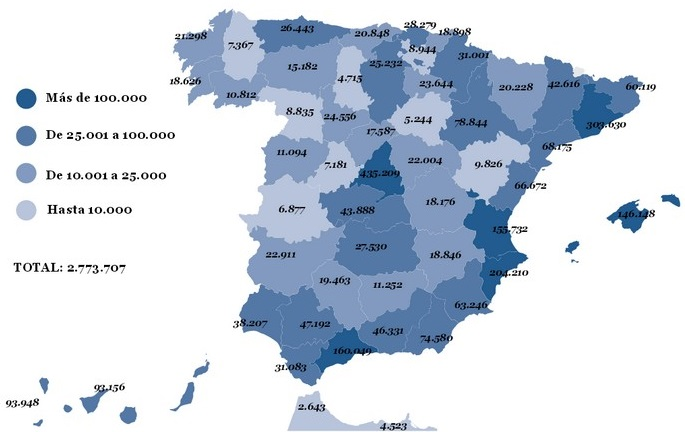
\includegraphics[width=10cm, height=8cm]{Images/Emigrantes.jpg} 
	\caption{Extranjeros de la Unión Europea por provincia en España }
\end{figure}

Por su parte América Latina centra sus estudios en las desigualdades económicas de la población. En la región existe una marcada diferencia entre las condiciones de vida de ricos y pobre en la mayoría de sus ciudades, debido en gran manera a su modelo de ciudad. Los pobres siguen conviviendo en las periferias y los ricos en “conos” de altos ingresos típicamente bien conectados con el centro comercial \cite{Janoschka2002ElNM}. Un estudio realizado en México resaltó como la diferenciación de la población según su condición socioeconómica es uno de los ejes más importantes y críticos de las marcadas diferencias en la sociedad contemporánea, y en particular en la mexicana \cite{Duhau2003DivisinSD}.

Los altos niveles de desigualdad como los que caracterizan a América Latina pueden conducir a la fragmentación de la sociedad como consecuencia del aislamiento de los sectores privilegiados y la exclusión de los más desfavorecidos \cite{Barry1998SocialES}. En este sentido la división social del espacio tiene como componente fundamental la característica de ser la expresión espacial de la estructura de clases o de la estratificación social \cite{Sarav2008MundosAS}. Es decir, si bien existen muchos posibles criterios de diferenciación social que a su vez podrían verse expresados en la estructura espacial, en una sociedad donde cobra una preeminencia absoluta la condición socio-económica para posicionar a los sujetos en la estructura social, esta preeminencia se ve reflejada en el espacio urbano.

De la mano de las marcadas diferencias socio-económicas de américa Latina existe otro problema de gran calibre: “La migración”, ya sea interna o externa. La migración se manifiesta tanto en las zonas de origen como en las zonas de destino, este efecto responde fundamentalmente a la magnitud y, sobre todo, a la selectividad de los flujos migratorios \cite{Vignoli2011MigracinIE}. Estudios realizados reflejan como la afluencia masiva de inmigrantes desde el campo, tiene grandes posibilidades de constituir un vasto sector de población marginada \cite{Elizaga1972MigracionesIE}. Un análisis realizado en varias ciudades importantes de la región, alerta sobre la necesidad de un nuevo enfoque en materia de políticas, sobre todo de las relacionadas con el incremento de la segregación que tiende a provocar la migración \cite{Vignoli2011MigracinIE}.




\subsection{Estudios de la Segregación en Cuba}

Los estudios acerca de la segregación residencial en la isla existen, pero aún son insuficientes. Principalmente orientados a las diferencias socio-económicas en el país y a raíz de la importancia del tema
en los últimos años ha habido un incremento en los estudios sobre el tema. Por su parte, el Centro de
Estudios Demográficos de la Universidad de La Habana (CEDEM) realiza investigaciones sobre cómo afectan las 
diferentes variables demográficas a la estructura poblacional cubana.  

Para entender la segregación social en Cuba y comprender cómo estos males afectan a los habitantes de la isla hay que partir de la base que cuba es un país abrumadoramente urbano. Según el censo del año 2000 el 76 \% de la población cubana era urbana y solo el 40 \% vivía en ciudades de más de 100000 habitantes \cite{CONEI2000}. Lo anterior destaca que un alto porcentaje de la población socializa en contextos urbanos complejos y en una red extendida de medianas ciudades, datos que ciertamente colocan el problema de la regionalización y de la fragmentación urbana en un escenario bastante complicado.

En los años 70 y 80 del pasado siglo la isla con la ayuda del campo socialista fue favorecida por políticas coherentes, basadas en una peculiar situación de recursos de manera abundante. De esta manera Cuba logró evitar en ese entonces alguno de los principales problemas que afrontó América Latina en ese período, como son las desigualdades territoriales extremas y la hipertrofia de las ciudades capitales. El país se organizaba en relación con un sistema de asentamientos humanos que según definió Concepción Álvarez en el año 2001, representaba: “la articulación espacial entre la producción y el consumo” \cite{AC2001}. Este esquema planteaba 4 niveles de asentamientos cada uno con funciones específicas en los esquemas regionales:

\begin{itemize}
	
	\item Una ciudad capital, que operaba con centro proveedor de servicios especializados y cabeza político/burocrática de la isla
	
	\item Una red de trece ciudades intermedias que funcionaban como capitales provinciales, con atribuciones económicas y administrativas sobre su territorio
	\item Un total de 142 ciudades menores (con poblaciones hasta 50000 habitantes), en su mayoría cabeceras municipales, eran proveedoras de servicios sociales y burocráticos.
	\item Una denomina franja base, compuesta por una población dispersa y una miríada de asentamientos urbanos y rurales, donde radicaba el 40 \% de la población de la isla.
	
	
	
\end{itemize}

Gráficamente se trataba de un ordenamiento jerárquico, estructurado desde la capital hasta la población dispersa. Las ciudades intermedias desempeñaban un papel decisivo en la canalización de las inversiones economías. El sistema era abastecido en su tope por los subsidios soviéticos los cuales eran distribuidos hasta la base. Cuba ha cambiado muy poco desde aquellos tiempos, pero la dinámica existente es sustancialmente diferente lo que empuja a una reestructuración espacial.

Tomando esta realidad como punto de partida existen varios análisis acerca situación de la vivienda y la segregación que la misma ha traído consigo, sobre todo en la comparación entorno al año 1959 \cite{Trefftz201150AD} \cite{Pascua2006LasZR}. De la mano de los trabajos que atacan los problemas de la segregación en Cuba de manera general están los que se centran en regiones más específicas. La Habana ha objetivo de varios estudios realizados principalmente enfocados a las diferencias económicas de los habitantes de la ciudad \cite{Herrero2007PlanesDR} \cite{Alfonso2008LaRE}.

\begin{figure}[htb]
	\centering
	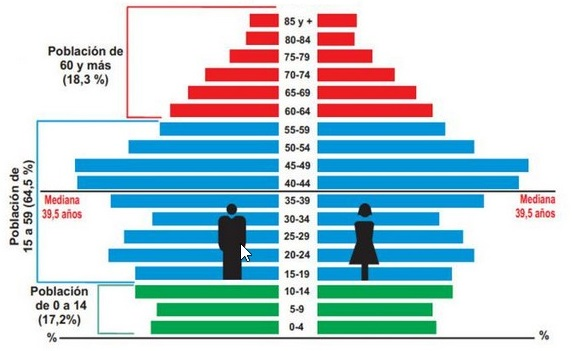
\includegraphics[width=8cm, height=7cm]{Images/CubaEnvejecimiento.jpg} 
	\caption{Estructura de población cubana por sexo y edades .Censo 2012 }
\end{figure}

Una problemática que demanda un análisis urgente en la realidad cubana es el envejecimiento \cite{CONEI2012}. Por una parte, el notable envejecimiento poblacional o demográfico y por otra la antigüedad de las viviendas en Cuba. El envejecimiento poblacional está determinado por disímiles factores: la baja natalidad, la emigración de personas jóvenes, y la elevada esperanza de vida en la isla \cite{Hernndez2015EnvejecimientoPE}. Como este fenómeno impacta directamente en la economía, ya que expresa una disminución en la fuerza laboral, ha sido ampliamente abordado en Cuba \cite{Prez2017ElED} \cite{R2020}. Sin embargo, la problemática del envejecimiento del casco urbanístico y rural cubano es mucho menos abordado. En Cuba el 33 \% de las viviendas tiene al menos 40 años, mientras que en ciudades como la Habana la cantidad de viviendas con al menos 40 años asciende al 51 \% de las viviendas. La investigación de este tema se hace particularmente necesaria, ya que el país se está viendo seriamente afectado por el envejecimiento de sus viviendas. El hecho de poder determinar los sectores más afectados por este fenómeno permite tomar decisiones más certeras, ofreciendo una mejor solución teniendo en cuenta la ubicación geográfica.



\subsubsection{La segregación en la era digital}

Los estudios sobre la segregación residencial en la era digital o de la información, donde todo lo que suene a tecnológico, a inteligencia artificial, a redes sociales se pone a la vanguardia; no pueden negar tales avances. Las nuevas tecnologías para el procesamiento, modelación y almacenamiento de datos proveen herramientas para un análisis más profundo y certero, creando un interés multidisciplinario e interdisciplinario por el análisis de los patrones residenciales y de los procesos sociales. 

El manejo de la llamada Big Data y la inteligencia artificial han permitido el análisis de mayores colecciones de datos \cite{man2018can}. En el año 2011 un artículo propuso la simulación de un modelo multiagente de las dinámicas de una ciudad, en la que sus habitantes cambian su comportamiento en función de las características de su vecindario y de la ciudad en general \cite{Feitosa2011MultiagentSF}. En el 2014, se lanzó una herramienta computacional capaz de 
calcular 43 índices de segregación, con una interfaz sencilla que solo requiere una colección datos geográficos y de población afín a la variable que se quiera analizar \cite{apparicio2014open}. 

En 2018 se realizó una investigación con datos provenientes de la base de datos de red Social Facebook como el sexo, la edad y el lugar de residencia para analizar segregación de género en una zona respecto a la posibilidad de acceso a internet \cite{Fatehkia2018UsingFA}. En la misma se emplearon modelos de correlación para determinar la relación existente entre las variables. Con la utilización de una base de datos geo-codificada y la utilización de modernas herramientas de la inteligencia artificial como la regresión multinomial, en el año 2020 se presentó un artículo que describía un análisis de la segregación residencial en el área de Ámsterdam, teniendo en cuenta salario, población inmigrante, nivel educacional y edad \cite{Boterman2020MultipleDO}. 

Gracias a las ventajas que ofrece la era digital en cuanto a la búsqueda de patrones en el procesamiento de datos, las trayectorias simples \cite{RandonFurling2018FromUS}, aplicadas sobre las ciudades se han convertido en enfoque bastante común en el análisis de la segregación. Las trayectorias simples permiten hacer un análisis multifocal, desde lo local, hasta toda la ciudad. Un estudio desarrollado en el Reino Unido basado en la utilización de trayectorias evidenció como las comunidades cerradas, que se han vuelto populares en las periferias de las ciudades de este país, contribuye y acentúan en gran manera la segregación residencial y alerta de la necesidad de políticas públicas que limite la creación de las mismas \cite{Atkinson2003FortressUG}. Las trayectorias también han sido un pilar fundamental para analizar los movimientos de los inmigrantes y analizar cómo influyen en los vecindarios a los que llegan \cite{Vogiazides2019MigrantsLR}. 

Otro enfoque es la utilización de algoritmos de agrupamiento para detectar si una ciudad o región presenta segregación. Un estudio sobre la ciudad española de Bilbao utilizó K-Means, para determinar la existencia de la segregación de ese territorio \cite{AguadoMoralejo2019AplicacinDU}. El grupo de investigación referente a la inteligencia artificial de la Universidad de la Habana ha realizado varios estudios para analizar la segregación residencial en la Habana tomando como referencia principal el artículo: “From urban segregation to spatial structure detection” \cite{RandonFurling2018FromUS}. Se realizó un trabajo con la utilización de algoritmos de agrupamiento para analiza la segregación respecto a la proporción de casas sociales y el envejecimiento poblacional de la Habana \cite{G2019}.

Estas investigaciones, sobre todo las desarrolladas por el grupo investigativo ge inteligencia artificial de la Universidad de la Habana, relacionadas con trayectorias y algoritmos de agrupamiento constituyen la base teórica para el desarrollo de esta tesis. Los resultados permiten realizar una comparación con los obtenidos en este trabajo.












  



\chapter{Metodologia} 

En el capítulo anterior se ilustró la importancia que tiene un análisis profundo sobre la segregación residencial debido a las devastas consecuencias que la misma provoca. En esta investigación, siguiendo con la serie de trabajos del Grupo de Inteligencia Artificial de la Universidad de la Habana, se abordó el tema de la segregación residencial tomando como objeto de estudio la ciudad de la Habana. El tema del envejecimiento del casco urbanístico en la Habana merece ser centro de más debates académicos, dada que la antigüedad de la ciudad está cerca de convertirse en un problema para el desarrollo de la misma. El estudio servirá de base para la toma de decisiones de las organizaciones pertinentes, así como constituirá los pilares para futuras investigaciones sobre el tema. En la investigación se utilizó el algoritmo de agrupamiento K-Means y una variación del método de trayectorias simples para sectorizar y agrupar los distritos en grupos con edades similares en cuanto a las viviendas. El utilizar ambos métodos sirvió a modo de comparación y validación de resultados acerca de la segregación existente en la Habana según la variable de estudio: “la edad de los distritos”, se entiende por la edad de un distrito como el promedio de las edades de sus edificaciones.


\section{Kmeans}

Las técnicas de agrupación de datos son análisis de datos descriptivos que se pueden aplicar a conjuntos de datos con múltiples variables para descubrir la estructura presente en los mismos. El agrupamiento de datos es una forma de clasificación no supervisada, ya que los grupos se forman evaluando similitudes y disimilitudes de características intrínsecas entre diferentes casos. La agrupación de los casos se basa en aquellas similitudes existentes y no sobre un criterio externo. Además, estas técnicas pueden ser útiles para conjuntos de datos de cualquier dimensión \cite{Morissette2013TheKC}.

K-means es un algoritmo de agrupamiento particional basado en la ubicación iterativa de los elementos en los clústeres en función de su cercanía con los centroides de los mismos \cite{MacQueen1967SomeMF}. El algoritmo es aplicado para separar en casos los elementos de un conjunto de datos en una partición del conjunto, grupos que no se sobreponen entre sí. El objetivo es producir grupos donde los elementos del mismo tengan un alto grado de similitud y a su vez que las similitudes entre dos grupos distintos sean pequeñas \cite{Hastie2001TheEO}.
K-Means incluye modelos de conectividad como métodos de agrupamiento jerárquico \cite{Morissette2013TheKC}. Estas técnicas tienen la ventaja de que no necesitan conocer el número de clústeres iniciales, pero son computacionalmente costosas por el hecho de que se basan en una matriz de disimilitud.

Otro objetivo fundamental de K-Means es la reducción de la complejidad de un conjunto de datos. En un artículo presentado en 1994, se disminuyó la complejidad de los datos utilizando letras para representar diferentes valores numéricos de las variables y se tomaban las letras como centro de los clústeres \cite{faber1994clustering}. Con el mismo corte teórico, disminuir la complexidad de los datos, K-Means es ampliamente utilizado como algoritmo iniciador para otros algoritmos computacionalmente costosos como son el caso de: Cuantificación vectorial(LVQ) y el algoritmo de mezclas gaussianas(GMM) \cite{Shannon2001AMT}.

Matemáticamente hablando K-Means es una aproximación de un modelo de mezcla normal con una estimación de las mezclas por máxima verosimilitud. La mezcla considera la pertenencia de un elemento a un clúster como una probabilidad de cada caso, basado en los promedios y covarianzas \cite{Symons1981ClusteringCA}.
Si la métrica escogida es las distancias euclidianas, el algoritmo K-Means se puede definir formalmente como un procedimiento que agrupa los elementos de una colección en diferentes clústeres de manera que se minimice la sumatoria del error cuadrático.
\begin{equation}
SSE = \sum_{j = 1}^{k} \sum_{x \in C_j} d(x,m_j)^2
\end{equation}
Con : 
\begin{itemize}
	
	\item 	$C_j es el j-ésimo clúster$ 
	
	\item $	m_j es el centroide del clúster  C_j $
	\item $	d(x, m_j) es la distancia entre el elemento x y el centroide m_j$
	\item k representa el número de clústeres
	
\end{itemize}
El algoritmo se describe con los siguientes pasos: 
\begin{enumerate}
	
	\item 	Escoger el número inicial de clústeres
	
	\item Escoger métrica
	\item Escoger de manera aleatoria k elementos de la colección, serán las semillas iniciales y actuarán como centroides en un primer momento, es decir, serán los centros de cada clúster 
	\item Asignar cada elemento de la colección al clúster que posea el centroide más cercano a él 
	\item Recomputar los centroides de cada clúster, utilizando los miembros de los mismos
	\item En caso de que el criterio de convergencia no se haya alcanzado, o sea, que el error cuadrático sea mínimo, repetir los pasos 4 y 5.
	
\end{enumerate}
Para aplicar K-Means al estudio de la segregación es necesario aterrizar ciertos conceptos. En esta investigación la ciudad estará dividida en distritos, que constituyen la unidad espacial base de este trabajo. Los próximos dos epígrafes describirán más a profundidad los procesos de inicialización del algoritmo: escoger el número de clústeres iniciales (paso 1 del algoritmo) y escoger la métrica (paso 2 del algoritmo). Una vez seleccionados el número de clústeres iniciales(K) y la métrica a utilizar se comienza con el algoritmo. Dado que los distritos son la unidad base en esta investigación en todo momento K valores estarán marcados como centroides de los clústeres. En un inicio estos K valores se seleccionan tomando los valores de la variable para K distritos aleatorios. Este proceso se realiza en el paso 3. En el paso 4 se recorre toda la ciudad y para cada distrito se le asigna el clúster más cercano. Entiéndase por clúster más cercano como el grupo de distritos de la ciudad centrados en el valor de la variable de estudio más próximo al valor que dicho distrito tiene para esa variable. Una vez realizada dicha asignación, en el paso 5 se re computan los centroides de cada grupo, promediando el valor de la variable de todos los distritos pertenecientes a un grupo determinado. Los pasos 4 y 5 se repetirán hasta que el error cuadrático sea mínimo. Lo que informalmente significa que cada distrito está asociado al clúster que minimiza la distancia entre ellos y maximiza la distancia con todos los demás clústeres. La distancia entre un distrito y un clúster se calcula aplicando la métrica seleccionada en el paso 2, utilizando como entrada a la métrica el valor de la variable para ese distrito y el centroide del clúster.
\subsection{Selección del número de clúster de K-Means}
Uno de los problemas a la hora de aplicar varios algoritmos de agrupamientos es que la obtención de buenos resultados muchas veces está ligada a la selección del número de clúster iniciales, K-Means no es la excepción. Aunque no existe un criterio objetivo para la selección de dicho número, que indiscutiblemente es un parámetro clave. En la literatura se registran diferentes métodos para seleccionarlo apropiadamente, entre ellos se destacan: GAP en su versión estadística (es un sistema algébrico computacional especialmente orientdo a la teoría de grupos), método Elbow, Coeficiente Silhouette, índice de Calinsky--Harabasz, índice Davies-Bouldin y Dendrograma. La implementación de estos métodos y un análisis detallado sobre los resultados emitidos por estos sirvió de base para una selección más acertada del parámetro referente al número de clústeres.
\subsubsection{El método Gap en su versión estadística}
El método Gap en su versión estadística fue desarrollado en la universidad de Stanford en el 2001 \cite{Tibshirani2000EstimatingTN}. La idea detrás del método es realmente sencilla, se centra en encontrar una manera para comparar que tan compactos son los clústeres con una distribución nula de los datos (una distribución sin clústeres obvios). Estima que el número óptimo de clústeres es el valor para el cual la compacidad de los clústeres en los datos originales se localiza lo más lejos posible en la curva de referencia.

Matemáticamente hablando:
\begin{equation}
	Gap_n(k)= E_n^{*}\{\log W_k \} - \log W_k
\end{equation}
Donde $E_n^{*}$ respresenta el valor esperado para una distribución nula en una muestra de tamaño n y $W_k$ es la medida de compacidad del clúster(WCS), que está basada en la suma del error cuadrático$(D_k)$:

\begin{equation}
D_k = \sum_{x_i \in C_k}\sum_{x_j \in C_k} d(x_i - x_j) 
\end{equation}
donde $"d"$ representa la distancia euclideana entre un par de puntos del clúster dado.

El WCS es el resultado de la suma de las inercias del algoritmo K-Means. Siendo la inercia la suma de las distancias al cuadrado de cada objeto del clúster a su centroide.
\begin{equation}
	Inercia = \sum_{i = 0}^{n} ||x_i - m_j||
\end{equation}

\subsubsection{El método Elbow }
El método Elbow goza de gran popularidad a consecuencia de su simplicidad. Utiliza los valores de WSS obtenidos para diferentes números de clústeres(k) y selecciona el “k” para el cual el cambio en el WSS comienza a disminuir. La idea detrás del método es que la variación antes mencionada cambia rápidamente para una cantidad pequeña de grupos y luego se ralentiza este cambio, dando lugar a la formación de una especie de codo en la curva. El punto del codo representa el número inicial de clúster óptimos según esta aproximación \cite{Yuan2019ResearchOK}. 
\subsubsection{El método del Coeficiente Silhouette  }
El método del Coeficiente Silhouette ilustra una manera de elegir el número de clústeres a partir del promedio del coeficiente de Silhoutte para cada punto. El coeficiente de Silhoutte para cada punto establece si para un punto determinado este pertenece al clúster que se le asignó:
\begin{itemize}
	\item S(i) cercano a 0 significa que el punto i esta entre dos clústeres
	\item S(i) cercano a -1, el punto “i” está mal asignado y es conveniente asignarlo a otro clúster
	\item S(i) cercano a 1, el punto “i” corresponde al clúster correcto
\end{itemize}
S(i) se define como:
\begin{equation}
S(i) = \frac{b(i) - a(i)}{max \{a(i),b(i)\} }
\end{equation}
donde b(i) es el promedio de las distancias mínimas de un punto i hacia el resto de los puntos en cualquier otro clúster y a(i) representa el promedio de la distancia del punto i hacia todos los puntos del mismo clúster \cite{Kaoungku2018TheSW}.
\subsubsection{El método del índice Calinski-Harabasz   }
El método del índice Calinski-Harabasz se basa en la siguiente comprensión sobre los clústeres:
\begin{enumerate}
	\item Son muy compactos
	\item Existe una buena distancia entre dos clústeres cualesquiera
\end{enumerate}
El índice se calcula dividiendo la varianza de la suma de los cuadrados de las distancias de cada objeto de la colección al centroide del clúster al que pertenece, entre la suma de los cuadrados de la distancia entre los centroide de los clústeres. Mientras mayor sea el índice mejor. La fórmula matemática que describe el proceso es:
\begin{equation}
	CH_k = \frac{BCSM}{k - 1} - \frac{n - k}{WCSM}
\end{equation}
donde k es el número de clústeres y n el número de elementos en los datos. La matriz de dispersión entre los clústeres(BCSM) calcula la separación entre los clústeres y la matriz de dispersión dentro del clúster(WCSM) calcula la compacidad de cada clúster \cite{Wang2019AnII}.

\subsubsection{El método del índice de Davies-Bouldin }
El método del índice de Davies-Bouldin al igual que índice de Calinski-Harabasz utiliza la separación y la unidad de los clústeres para su análisis. Se define como:
\begin{equation}
DB = \frac{1}{k} - \sum_{i = 1}^{k} max_{j \neq i}(\frac{\sigma_i + \sigma_j}{d(c_i,c_j)})
\end{equation}
donde  k  es el número de clústeres y $\sigma_i$ es la distancia promedio de todos los puntos del cluster “i” al centroide $(c_i)$ del mismo \cite{Petrovic2006ACB}.
\subsubsection{El método Dendrograma }
El método Dendrograma es una técnica asociada únicamente a los métodos de aglomeración jerárquica. Un método agrupamiento basado en aglomeración jerárquica en un inicio considera cada punto como un clúster separado y comienza a unir los puntos a los clústeres jerárquicamente basándose en las distancias entre ellos. 
Para obtener el número óptimo de clústeres se utiliza un dendrograma que muestra la secuencia de mezclas y separaciones de cada clúster. Cuando se mezclan dos clústeres, el dendrograma los une y les asigna como valor resultante de la unión la distancia entre ambos clústeres.


\subsection{Selección de la métrica}
La selección de la métrica apropiada depende del problema en cuestión. De manera general la similitud entre los elementos de un conjunto de datos, en los algoritmos de agrupamiento se toma como una función de proximidad. De esta manera los elementos más cercanos entre sí, acorde a una o varias variables, en el espacio de entrada son considerados más similares. La métrica más común para computar la proximidad es la distancia euclidiana [13]: 
\begin{equation}
	dE = \sqrt{\sum_{i}^{k}(c_i -x_i)^2}
\end{equation}
Donde “c” es el centro del clúster, “x” el elemento que se está analizando en ese momento y k corresponde al número de dimensiones con que cuentan los datos. Otras métricas usadas en la literatura son: “Distancia euclidiana al cuadrado”, “Distancia manhattan”, “Máxima distancia entre los atributos de un vector” y “Distancia Mahalanobis”. 
\subsection{Ventajas y desventajas de K-Means}
K-means es realmente un algoritmo fácil de comprender e implementar. Su complejidad temporal es O(n*t*k), donde n es la cardinalidad del conjunto sobre el que se aplica, “k” el número de clústeres y t el número de operaciones, como “k” y “t” son pequeños, se considera un algoritmo lineal. Por otra parte, es necesario destacar que este algoritmo solo se puede aplicar si la media de los datos está definida. Es necesario especificar el número “k” referente a la cantidad de clúster. Por último, el algoritmo tiene malos resultados para los puntos aislados. A pesar de todas sus marcadas limitaciones y que no se puede tomar como un algoritmo de agrupamiento de carácter general, sigue siendo uno de los más utilizados en la literatura debido a su simplicidad \cite{Morissette2013TheKC}.

\section{Trayectorias Simples}
El empleo de trayectorias simples es una herramienta moderna y poderosa para investigar las estructuras espaciales en una determinada ciudad. Se tiene conocimiento de que eventualmente, todas las trayectorias locales convergerán hacia un mismo valor. Dependiendo de si la convergencia se logra muy rápidamente o muy lentamente, esto significaría que esas unidades espaciales de las que parten esas trayectorias difieren del comportamiento medio de la ciudad para esa variable, lo que implica un grado de aislamiento. En general, las trayectorias describen cuán rápido puede una estructura individual comportarse como toda la ciudad. El análisis profundo de la similitud de entre cada estructura individual con toda la ciudad permite determinar el comportamiento de las variables de la ciudad para determinar si existe o no segregación.

Una trayectoria consiste en un camino de Hamilton partiendo de una unidad censal, camino que recorre toda la ciudad sin repetir ninguna unidad censal \cite{RandonFurling2018FromUS}. Se puede definir como la suma acumulativa que la variable de estudio tiene en cada estructura individual o unidad censal. El orden en que se recorren las unidades censales se hace atendiendo a los valores de distancia euclidiana entre cada uno de ellos \cite{Armas2020AnlisisDS}. Sin embargo, en esta investigación se realizó una pequeña modificación con respecto al orden de recorrido de las unidades censales. Se recorrieron con respecto a una ordenación de los mismos, a partir del valor de la variable de estudio en la unidad censal inicial.

Matemáticamente hablando una trayectoria simple $t= \{ U_i,1 \leq i \leq N \} $ , donde $U_i$ = ( $coord_i; X_i$  ) , donde i = 1...N es el índice de la unidad censal, N es el número de bloques censales, $coord_i$ son las coordenadas del centroide de i y $X_i$ valor de la variable estadística presente en la unidad censal  i. 

\subsection{Ventajas y desventajas de Trayectorias Simples}
Trayectorias Simples es un algoritmo de fácil de comprender e implementar. Su complejidad temporal es $O(n^2)$, donde n es la cardinalidad del conjunto sobre el que se aplica. Por otra parte, es necesario destacar que este algoritmo solo se puede aplicar en conjuntos de datos cuantitativos. Por último, el algoritmo original presenta dos limitaciones fundamentales   su recorrido únicamente tiene en cuenta las distancias euclidianas entre los diferentes puntos de la ciudad y, para cada trayectoria, se analiza el comportamiento de una única variable. 
\subsection{Modificaciones al método de Trayectorias simples}
En la búsqueda de mejorar las limitaciones del método de Trayectorias simples en esta investigación se implementaron una serie de modificaciones. El hecho de que el orden de una trayectoria siempre fuera tomado por la distancia geográfica entre los distritos no permitía realizar un recorrido en ordenado de los distritos según el valor de la variable de estudio. Se implementó que la distancia entre las unidades censales de la ciudad se mida en cuanto al valor de la variable con lo que se esperan obtener mejores resultados. Para posibilitar recorridos que tengan en cuenta múltiples variables se sustituyo $X_i$ en el algoritmo de trayectorias simples por un vector con los valores de todas las variables estadísticas presentes en esa unidad censal.
\subsection{Propuestas con el método de Trayectorias simples}
En el método de trayectorias simples, existe lo que en la literatura se conoce como radio de convergencia [14], que no es más que un punto donde cada trayectoria entra a un intervalo de confianza (en este caso se utilizó $\pm$0.1) alrededor de la tasa promedio de las viviendas construidas antes del 1959 en la ciudad. Con esta definición de base se desarrolló un método para estimar el número de clústeres óptimo para utilizar el algoritmo Kmeans. El método consta de un funcionamiento sencillo: computar el radio de convergencia para cada trayectoria y posteriormente tomando estos datos como entradas utilizar el algoritmo Dendograma previamente descrito en este trabajo. Queda propuesto para trabajos futuros una mejor selección del intervalo de confianza.

%===================================================================================
% Chapter: Marco Experimental
%===================================================================================

\chapter{Experimentación y Resultados} 
El objetivo de este capítulo es realizar la validación de la metodología que se presentó en este estudio se conformaron tres experimentos. El primero pretende estimar el número de clústeres óptimo para Kmeans, un parámetro sumamente importante para alcanzar buenos resultados. El segundo plantea una comparación entre el método de trayectorias simples y el método de trayectorias con las modificaciones propuestas. Por último, se diseñó un experimento a modo de comparación entre los algoritmos: Kmeas y Trayectorias Simples Modificado.
Los datos sobre los que se ejecutan los experimentos son descritos en el siguiente epígrafe. Para la realización de estas pruebas se utiliza una máquina con las siguientes características: Intel i7-660U,16 gb RAM.

\section{Datos}
Un aspecto fundamental en el estudio de la segregación es el procesamiento de los datos. Un análisis concreto de los mismos brinda información más que necesaria en base a criterios rigurosos que pueden influir en la toma de decisiones a la hora de determinar la existencia o no de segregación en un territorio o población determinada. Para la detección de la segregación en la Habana, se cuenta con datos provenientes de dos fuentes fundamentales: Oficina Nacional de Estadísticas e Información de la República de Cuba (ONEI) y el grupo empresarial GEOCUBA. De la ONEI se obtuvo el censo poblacional realizado en el 2012, que aporta un gran número de características y variables para realizar un análisis profundo sobre la población y la vivienda en la Habana. De GeoCuba se adquirió una base de datos que contiene datos geoespaciales para cada entidad del estudio.

Lograr establecer una relación entre ambas fuentes de datos no fue una tarea sencilla. Para encontrar un punto común entre ambas fuentes, se decidió asociar los datos en torno a distritos (conjunto de manzanas), que serán la unidad básica de medida en el estudio de segregación para ambos algoritmos. Vale destacar que, aunque la mayor parte de estudios poblacionales realizados en Cuba utilizan las circunscripciones como unidad base, la elección de los distritos no resulta una elección aleatoria. Por una parte, no se disponía de la ubicación geoespacial para las circunscripciones, unido a que los antecedentes a este trabajo, están realizados sobre la ciudad de Paris, lugar donde se toma con unidad base los IRIS. Un Iris es equivalente a la unión de varios distritos. 

La información referente al censo poblacional de la ONEI se reagrupó en torno a los distritos de cada municipio, obteniendo un cúmulo de variables muy importantes para el análisis; entre ellas: la cantidad de viviendas, la cantidad de población, clasificaciones de la población en cuanto al sexo, color y grupos de edades, por solo mencionar unas pocas. Este estudio se enfoca en el análisis de la variable “Edad de las viviendas”, pero el trabajo realizado abre las puertas al grupo de investigación para el análisis del resto de las variables en futuros trabajos. La geolocalización de los distritos presentó desafíos interesantes pues la base de datos de GEOCUBA tiene como unidad básica las manzanas. Para poder estimar la ubicación de los distritos fue necesario el siguiente análisis: en todo municipio existen múltiples distritos, los que a su vez están formados por múltiples manzanas, o sea, que si para cada distrito en un determinado municipio se cuenta con la geolocalización de cada una de las manzanas que pertenecen al mismo se puede aproximar su ubicación. Lo descrito anteriormente se realizó de la siguiente forma:
\begin{itemize}
	\item De los datos de la ONEI determinar el municipio del distrito.
	\item De los datos de la ONEI seleccionar todas las manzanas que forman parte del distrito.
	\item Para cada manzana perteneciente a dicho distrito buscar sus posibles coordenadas en la base de datos de GEOCUBA, recordar que para un mismo identificador de manzana en la base de datos de GEOCUBA existen varias entradas.
	\item Con todas las posibles coordenadas para una determinada manzana seleccionar aquella que pertenezca al municipio en cuestión, es necesario destacar que la pertenencia se tomó parcialmente pues los polígonos asociados a manzanas y los polígonos asociados a los municipios procedían de tablas diferentes lo que provocó cierta incongruencia en los datos. Resumiendo, se asumió que una manzana pertenecía a un municipio si el 60\% de los puntos del polígono que la describía estaban dentro del polígono que describía al municipio.
	\item Con los datos referentes a la ubicación de todas las manzanas de un distrito computar el centroide.
\end{itemize}

El resultado de todo el proceso fue un archivo de tipo “json” que almacena información relevante de un gran número de distritos de la Habana, convirtiéndose en la base de información fundamental para el estudio. 



\section{Experimento 1: Selección del número de clústeres para Kmeans}\label{Experimento1}
El número óptimo de clústeres para Kmeans es posiblemente el parámetro fundamental a la hora de aplicar el algoritmo. Es por esta razón, que se hizo necesario un estudio sobre los métodos empleados para estimar el número de clústeres. En este experimento se analizó los resultados para los métodos descritos en el capítulo anterior.

\subsection{Gap en su versión estadística}
Como se describe en el capítulo anterior, este método devuelve como posible k, el valor q maximiza las diferencias entre la compacidad de los datos originales con los datos agrupados con una distribución sin clústeres obvios. Para los datos analizados se obtiene k=29. Es decir, sugiere la formación de 29 clústeres. (ver Figura [ \ref*{fig:Gap} ])


\begin{figure}[h!]
	\centering
	\includegraphics[width=8cm, height=5cm]{Images/Gap_Static.jpg} 
	\caption{Gap en su versión estadística }
	\label{fig:Gap}
\end{figure}

\subsection{Método Elbow}
Este método es un método apreciativo. Se encarga de estimar para qué valor la suma de las inercias del algoritmo K-Means comienza a disminuir. En este caso, el punto, donde la variación antes mencionada cambia rápidamente para una cantidad pequeña de grupos y luego se ralentiza este cambio, dando lugar a la formación de una especie de codo en la curva es para k = 6. (ver Figura [ \ref*{fig:Elbow} ])

\begin{figure}[h!]
	\centering
	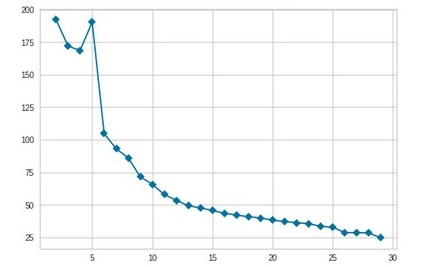
\includegraphics[width=8cm, height=5cm]{Images/Elbow.jpg} 
	\caption{Método Elbow }
	\label{fig:Elbow}
\end{figure}

\subsection{El método del Coeficiente Silhouette}
Partiendo de la metodología el coeficiente Silhoutte de una entidad es 1 si pertenece al clúster indicado. En otras palabras, a mayor valor global del coeficiente Silhoutte hace que la pertenencia de cada entidad al clúster determinado sea la mayor. En este caso particular se alcanza para k = 12. (ver Figura [ \ref*{fig:SCoe1} ])

\begin{figure}[h!]
	\centering
	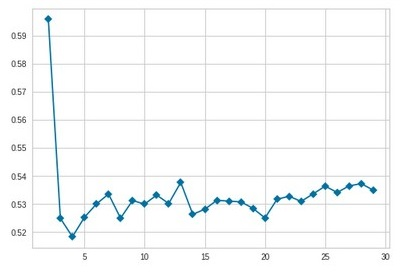
\includegraphics[width=8cm, height=5cm]{Images/SCoe1.jpg} 
	\caption{Método del Coeficiente Silhouette}
	\label{fig:SCoe1}
\end{figure}

\subsection{El método del Coeficiente Silhouette segunda variante}
La idea con esta segunda variante del método es más apreciativa. En la figura [ \ref{fig:SCoe2} ] se observa una línea roja discontinua, que marca el valor de compacidad para cada caso, si para algún k (número de clústeres iniciales), algún clúster (las figuras de colores) no alcanza el valor de compacidad ese k no debe ser escogido. Esta primera regla no se cumple en ninguno de los casos, por lo que se prosiguió a la siguiente regla en la metodología: escoger el k para el cuál las formas de los clústeres tengan la distribución más uniforme posible, o sea, que sus figuras sean similares. Como se puede apreciar en la figura [ \ref{fig:SCoe2} ], los clústeres más uniformes se alcanzan para K = 3.

\begin{figure}[h!]
	\centering
	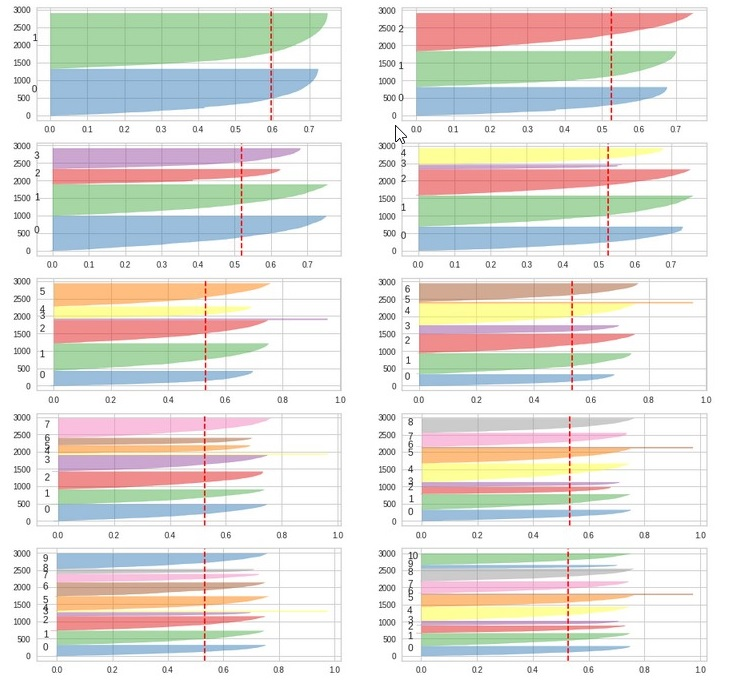
\includegraphics[width=8cm, height=10cm]{Images/SCoe2.jpg} 
	\caption{Método del Coeficiente Silhouette}
	\label{fig:SCoe2}
\end{figure}
\subsection{El método del índice Calinski-Harabasz}
Este algoritmo establece que a mayor valor del índice de Calinski-Harabasz es una mejor estimación para el número inicial de clústeres, ya que la misma garantiza una mayor compacidad de los clústeres. En este caso se seleccionó k = 29, como se observa en la figura [ \ref*{fig:CI} ], para 29 clústeres se alcanza el mayor valor para el índice de Calinski-Harabasz.


\begin{figure}[h!]
	\centering
	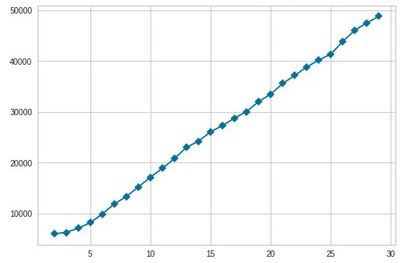
\includegraphics[width=8cm, height=5cm]{Images/CIndex.jpg} 
	\caption{Índice Calinski-Harabasz}
	\label{fig:CI}
\end{figure}
\subsection{El método del índice de Davies-Bouldin}
Este método tiene un principio muy similar al índice Calinski-Harabasz y al coeficiente Silhouette, dado que captura tanto la compacidad como la separación de los clústeres. A diferencia de ambos métodos mencionados a menor valor del índice de Davies-Bouldin, la literatura establece que se alcanzan mejores resultados. En este trabajo se seleccionó k = 12, dado que como se observa en la figura [ \ref{fig:DI} ], para 12 clústeres se alcanza el menor valor para el índice de Davies-Bouldin.

\begin{figure}[h!]
	\centering
	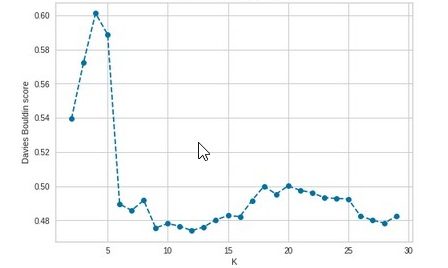
\includegraphics[width=8cm, height=5cm]{Images/DIndex.jpg} 
	\caption{Índice Davies-Bouldin}
	\label{fig:DI}
\end{figure}
\subsection{El método Dendrograma}
Dado que un dendrograma es una representación gráfica de datos en forma de árbol, dónde los datos se agrupan en subcategorías. En este método se toma el número de subcategorías como el número óptimo de clústeres, se obtuvo k = 3. Se puede apreciar en la figura [ \ref*{fig:Dend} ] donde cada categoría está marcada con un color solo aparecen tres colores, dictaminando que en el árbol de los datos analizados hay tres subcategorías presentes, o sea, que la mejor distribución de los datos sería en tres clústeres.

\begin{figure}[h!]
	\centering
	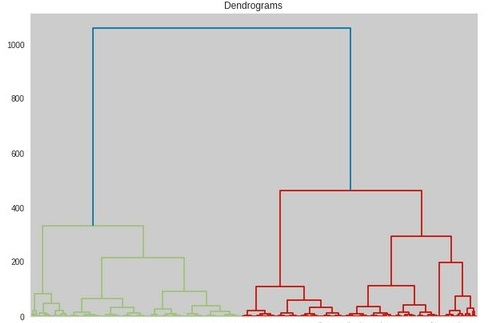
\includegraphics[width=8cm, height=6cm]{Images/Dendograma.jpg} 
	\caption{Método Dendrograma}
	\label{fig:Dend}
\end{figure}

\subsection{Resumen de los métodos}

\begin{table}[h!]
	 \begin{threeparttable}
	\begin{center}
		\begin{tabular}{| l | r | c |}
			\hline
			Método & K \tnote{1}  & Tiempo de Ejecución(Segundos) \\ \hline
			Gap en su versión estadística & 29 & 60 \\
			Elbow & 6 & 7 \\
			Coeficiente Silhouette & 13 & 11 \\
			Coeficiente Silhouette(2) & 3 & 6 \\
			Índice Calinski-Harabasz & 29 & 7 \\
			Índice de Davies-Bouldin & 12 & 6 \\
			Dendrograma & 3 & 14 \\
			Moda & 3 & -\\
			Promedio & 13 & - \\ \hline
		\end{tabular}
		\begin{tablenotes}
		\item[1] K : Representa el número de clústeres óptimo para Kmeans.
		
		\end{tablenotes}  
		\caption{Número de Clústeres Óptimo vs Tiempo de Ejecución}
		\label{tab:resumenMetodos}
	\end{center}
	 \end{threeparttable}
\end{table}



\begin{figure}[h!]
	\centering
	
	\begin{subfigure}[b]{0.49\linewidth}
		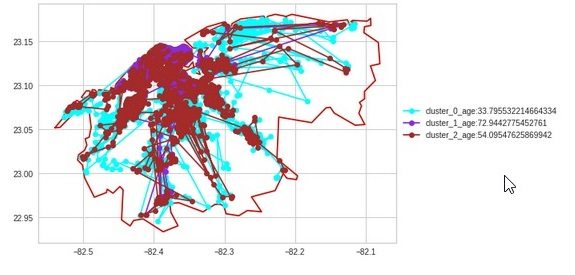
\includegraphics[width=\linewidth, height=3cm]{Images/3.jpg}
		\caption{Kmeans tres Clústeres}
	\end{subfigure}
	\begin{subfigure}[b]{0.49\linewidth}
		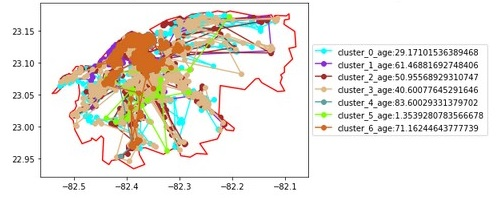
\includegraphics[width=\linewidth, height=3cm]{Images/6.jpg}
		\caption{Kmeans seis Clústeres}
	\end{subfigure}
	\begin{subfigure}[b]{0.49\linewidth}
		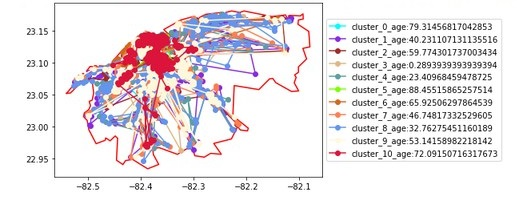
\includegraphics[width=\linewidth, height=3cm]{Images/11.jpg}
		\caption{Kmeans 11 Clústeres}
	\end{subfigure}
	\begin{subfigure}[b]{0.49\linewidth}
		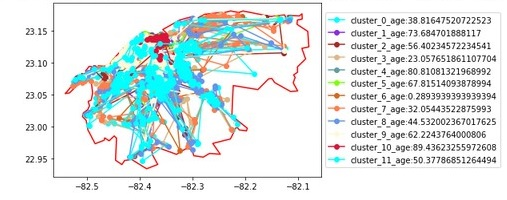
\includegraphics[width=\linewidth, height=3cm]{Images/12.jpg}
		\caption{Kmeans 12 Clústeres}
	\end{subfigure}
	\begin{subfigure}[b]{0.49\linewidth}
		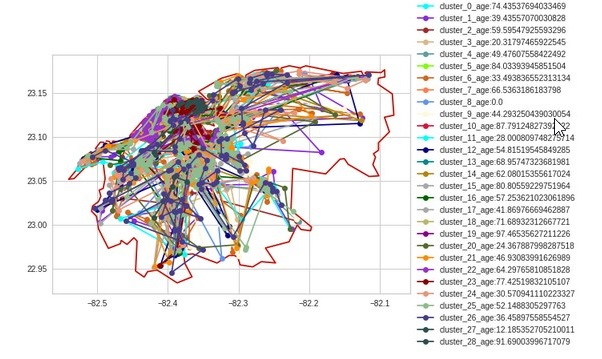
\includegraphics[width=\linewidth, height=3cm]{Images/29.jpg}
		\caption{Kmeans 29 Clústeres}
	\end{subfigure}
	\caption{Distribución de la Habana según Kmeans}
	\label{fig:Kmeans}
\end{figure}

El análisis realizado se identificó K = 3 como el número de clústeres óptimo para el algoritmo de Kmeans, para el conjunto de datos estudiados. Por un lado, es el valor de la moda de todos los algoritmos estudiados para la estimación de dicho parámetro y por otro resultó ser el más descriptivo en cuanto a las diferencias de los clústeres. Esto se puede apreciar claramente en las imágenes asociadas a cada uno de los resultados de los métodos donde a mayor número de clústeres menor las diferencias entre el valor de su centroide, lo que impedía tomar decisiones certeras. La figura [ \ref{fig:Conc} ], muestra el resultado final de aplicar el algoritmo k means con k =3 y el valor de sus centroides.

\begin{figure}[h!]
	\centering
	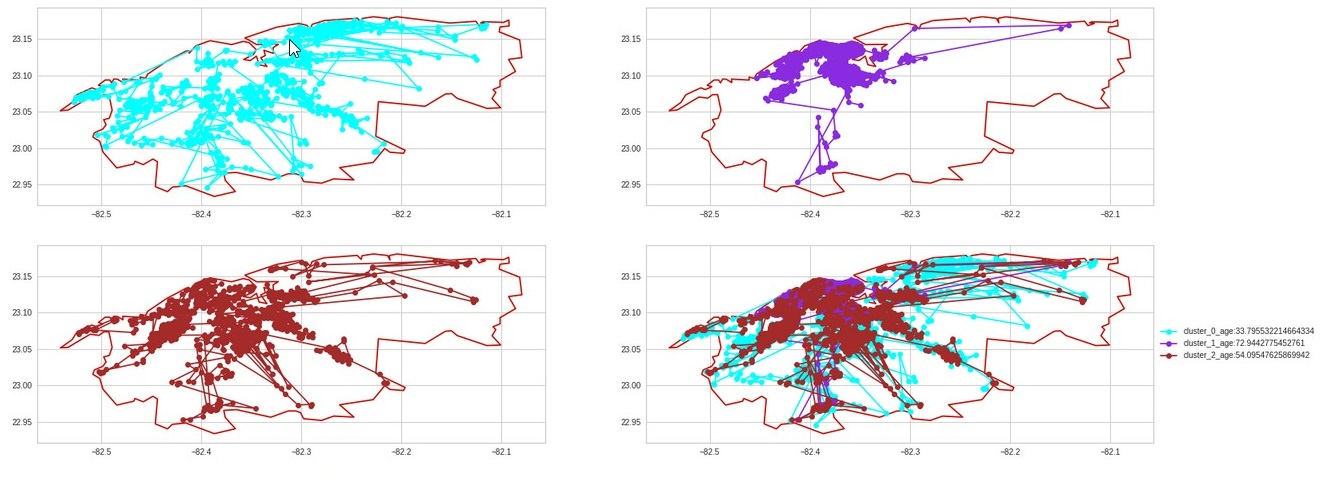
\includegraphics[width=15cm, height=7cm]{Images/Conclusion.jpg} 
	\caption{Habana dividida en tres clústeres}
	\label{fig:Conc}
\end{figure}

En muchas ocasiones un análisis desde lo local, es fundamental en el estudio de una problemática. El estudio de la segregación en la habana con respecto a su casco urbanístico no es la excepción. Existen municipios que se comportan como la ciudad que ya de por si marca un envejecimiento de las viviendas preocupante mientras que existen otros como es el caso de la Habana Vieja que sus promedios de edades son muy superiores a la media. Sin embargo, para la periferia de la ciudad municipios como el Cotorro o Boyeros son realmente “jóvenes” si de antigüedad de sus viviendas se trata.




\begin{figure}[h!]
	\centering
	\begin{subfigure}[b]{0.49\linewidth}
		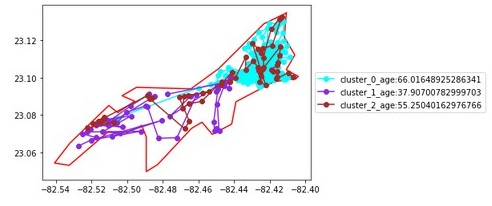
\includegraphics[width=\linewidth, height=3cm]{Images/Playa.jpg}
		\caption{Playa}
	\end{subfigure}
	\begin{subfigure}[b]{0.49\linewidth}
		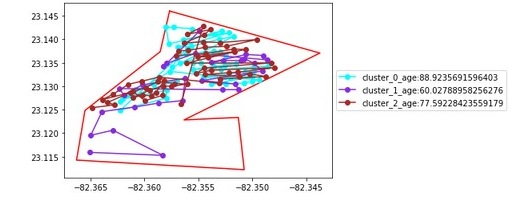
\includegraphics[width=\linewidth, height=3cm]{Images/HabV.jpg}
		\caption{Habana Vieja}
	\end{subfigure}
	\begin{subfigure}[b]{0.49\linewidth}
		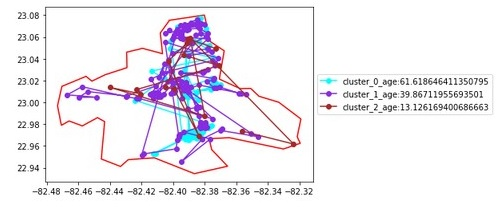
\includegraphics[width=\linewidth, height=3cm]{Images/Boyeros.jpg}
		\caption{Boyeros}
	\end{subfigure}
	\caption{Municipios de la Habana}
	\label{fig:muns}
	
\end{figure}

Los clústeres obtenidos para el resto de los municipios pueden consultarse en el Anexo [ \ref{chapter:Anexo} ].

\newpage
Queda propuesto para trabajos posteriores realizar un análisis más profundo a nivel de localidad para los distintos municipios de la Habana. Estudio futuro que espera aportar nuevos y determinantes argumentos para establecer una comparación más a fondo entre lo local y lo global(municipio-ciudad).
\newpage
\section{Experimento 2: Trayectorias Simples – Trayectorias simples modificadas}
Los resultados de ambas metodologías para los datos de la proporción de las viviendas de antes del 1959 con respecto al total de viviendas en la Habana, se compararon en cuanto al tiempo de ejecución y el recorrido descrito sobre el mapa.

\begin{table}[h!]
	\begin{center}
		\begin{tabular}{| l | c | c |}
			\hline
			Método & Una Trayectoria & Todas las Trayectorias \\ \hline
			Trayectorias Simples & - & - \\
			Trayectorias simples modificadas & - & - \\ \hline
		
		\end{tabular}
		\caption{Tiempo de Ejecución de las Trayectorias}
		\label{tab:resumenTrayectorias}
	\end{center}
\end{table}

\begin{figure}[h!]
	\centering
	\begin{subfigure}[b]{0.49\linewidth}
		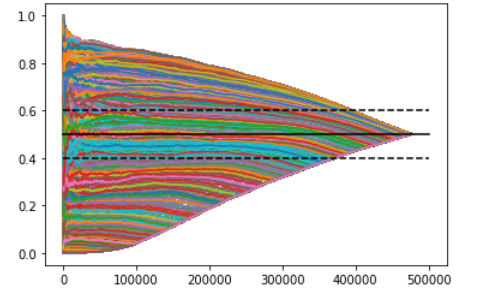
\includegraphics[width=\linewidth, height=3cm]{Images/TrayecCon.png}
		\caption{Trayectorias Modificadas}
	\end{subfigure}
	\begin{subfigure}[b]{0.49\linewidth}
		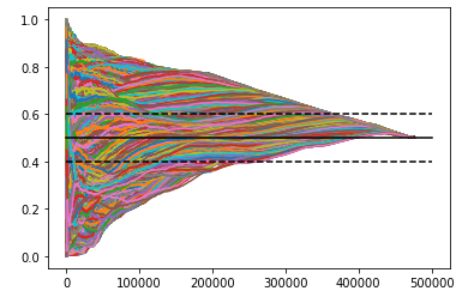
\includegraphics[width=\linewidth, height=3cm]{Images/ValueTray.png}
		\caption{Trayectorias Simples}
	\end{subfigure}

	\caption{Trayectorias de la Habana}
	\label{fig:trayectorias}
\end{figure}

La imagen [ \ref{fig:trayectorias} ] describen el conjunto de todas las trayectorias para ambas metodologías. Las fluctuaciones en las figuras determinan qué tan rápido convergen las trayectorias.

\newpage

Un análisis desde lo local puede resultar mucho más provechoso para analizar las diferencias entre ambos métodos de trayectorias. Las figura [ \ref{fig:Onetrayectorias} ] muestran el comportamiento de una única trayectoria, que parte desde el mismo distrito utilizando ambos métodos de trayectorias. En la figura [ \ref{fig:OnetrayectoriasM} ] se muestra una convergencia más lineal pues el recorrido en orden del valor de la variable. En la figura [ \ref{fig:OnetrayectoriasS} ] se muestra una convergencia menos lineal esto se debe a que el recorrido se realiza por cercanía lo que implica que varía grandemente el valor que toma la variable de estudio independientemente de la cercanía.

\begin{figure}[h!]
	\centering
	\begin{subfigure}[b]{0.49\linewidth}
		\includegraphics[width=\linewidth, height=3cm]{Images/OneTrayecV.png}
		\caption{Trayectorias Modificadas}
		\label{fig:OnetrayectoriasM}
	\end{subfigure}
	\begin{subfigure}[b]{0.49\linewidth}
		\includegraphics[width=\linewidth, height=3cm]{Images/OneTrayecD.png}
		\caption{Trayectorias Simples}
		\label{fig:OnetrayectoriasS}
	\end{subfigure}
	
	\caption{Única Trayectoria}
	\label{fig:Onetrayectorias}
\end{figure}

\subsection{Recorrido en el mapa }

\begin{figure}[h!]
	\centering
	\begin{subfigure}[b]{0.49\linewidth}
		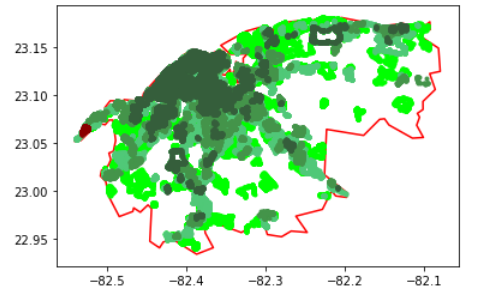
\includegraphics[width=\linewidth, height=3cm]{Images/TrayecVa.png}
		\caption{Trayectorias Modificadas}
		\label{fig:TrayecVa}
	\end{subfigure}
	\begin{subfigure}[b]{0.49\linewidth}
		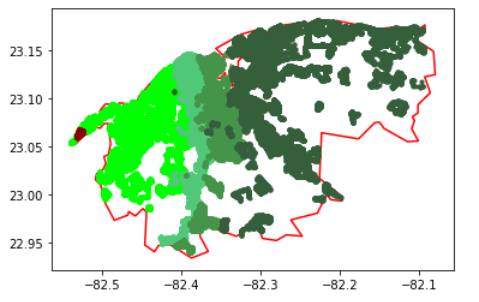
\includegraphics[width=\linewidth, height=3cm]{Images/TrayecDis.png}
		\caption{Trayectorias Simples}
		\label{fig:TrayecDis}
	\end{subfigure}
	
	\caption{Recorrido por el mapa}
	\label{fig:RecorridoTrayectorias}
\end{figure}

La figura [ \ref{fig:RecorridoTrayectorias} ]  muestran el recorrido en el mapa para ambas metodologías. El método de trayectorias simples muestra un recorrido claramente por distancia geográfica entre distritos [ \ref{fig:TrayecDis} ], mientras que el método de trayectorias modificadas [ \ref{fig:TrayecVa} ] hace un recorrido desde la periferia hasta el interior. Este comportamiento del recorrido del método de trayectorias modificadas, se debe en gran medida al distrito seleccionado. En este caso se seleccionó un distrito de la periferia, marcado con un punto rojo, se puede observar como la trayectoria primero recorre la periferia de la ciudad y luego se va adentrando en la misma. El orden del recorrido está dado por el grado de intensidad del color verde, mientras más oscuro más tarde se recorrió. Lo que ratifica que los municipios de la periferia tienen edificaciones más jóvenes.

\section{Experimento 3: Comparación Kmeans – Trajectorias Simples Modificado}
El objetivo principal de esta comparación es analizar la distribución realizada por ambos algoritmos a los distritos de la Habana. Para ello un punto inicial es lograr obtener a partir del método de trayectorias el número de clústeres óptimo(K) para Kmeans. El método propuesto para realizar dicha tarea, propone una estimación del K a partir del momento de entrada al intervalo de confianza de cada trayectoria.

\begin{figure}[h!]
	\centering
	\begin{subfigure}[b]{0.6\linewidth}
		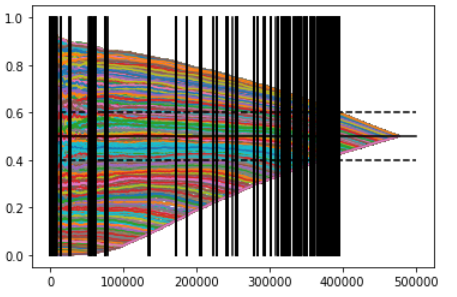
\includegraphics[width=\linewidth, height=5cm]{Images/Convergency2.png}
		\caption{Trayectorias Modificadas Convergencia}
		\label{fig:Convergency2}
	\end{subfigure}
	\begin{subfigure}[b]{0.6\linewidth}
		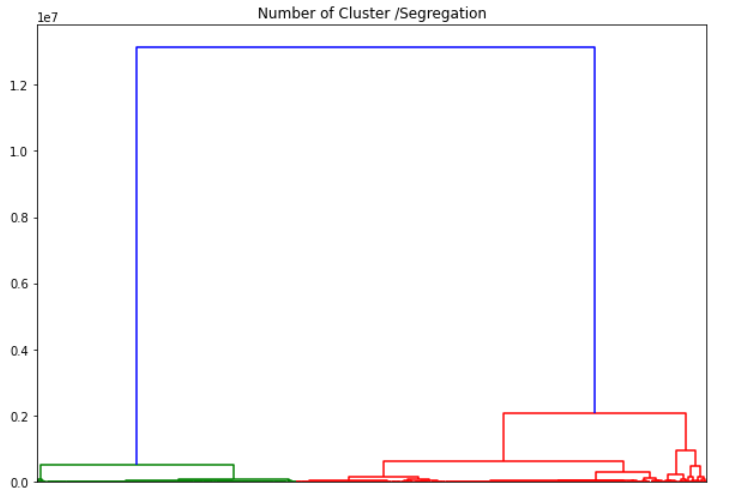
\includegraphics[width=\linewidth, height=5cm]{Images/ConvergenciaTrayec.png}
		\caption{Dendograma de Convergencias}
		\label{fig:ConvergenciaTrayec}
	\end{subfigure}
	
	\caption{Convergencia de Trayectorias}
	\label{fig:TrayectoriasConV}
\end{figure}

Como se puede apreciar en la figura [ \ref{fig:TrayectoriasConV} ] el resultado del método propuesto fue k = 3. La entrada del método fueron los datos de la proporción de las viviendas de antes del 1959 con respecto al total de viviendas en la Habana. El resultado corrobora la elección realizada en el primer experimento.

En este punto se hace necesaria la siguiente interrogante: \textbf{¿Si ambos métodos dividen la ciudad en tres clústeres, son acaso los mismos?}

\begin{figure}[h!]
	\centering
	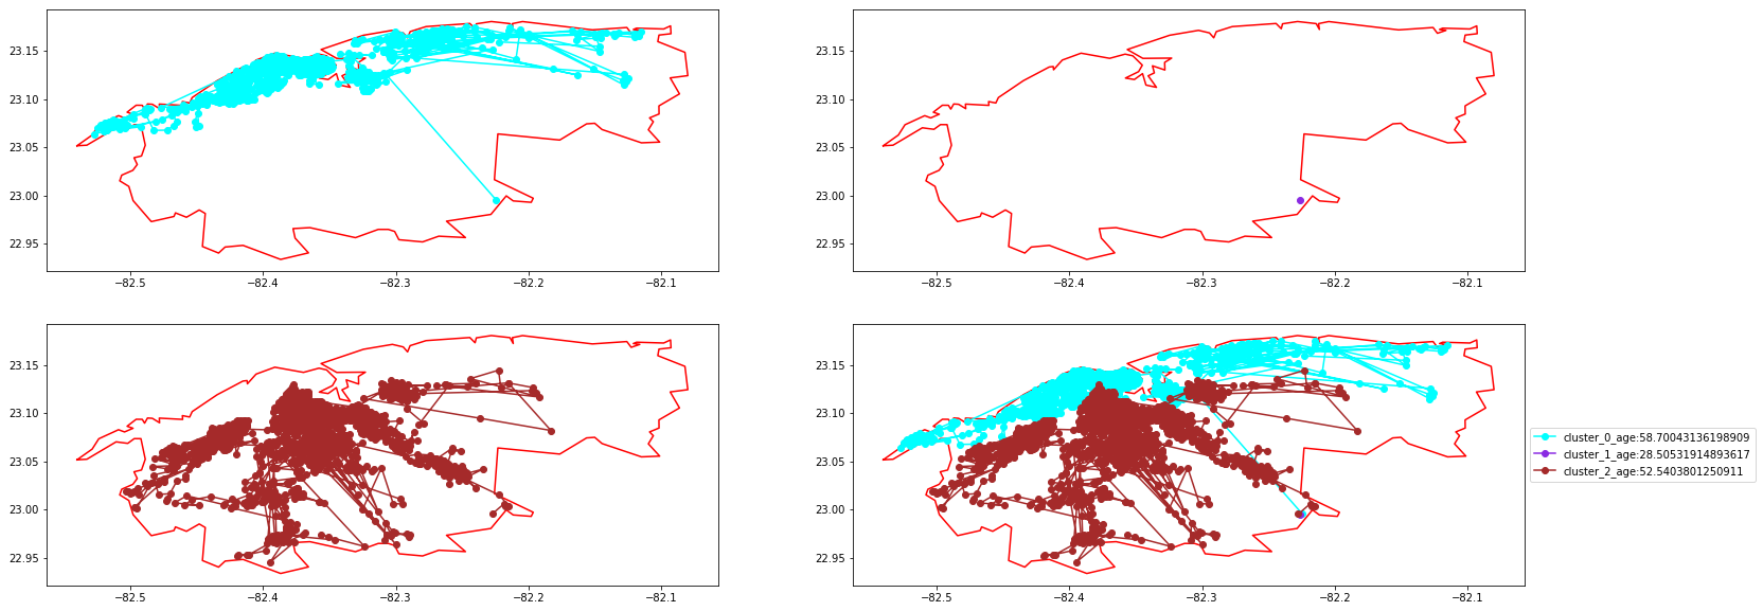
\includegraphics[width=15cm, height=7cm]{Images/Hab3KTrayec.png}
	\caption{Habana dividida por el método de trayectorias}
	\label{fig:Hab3KTrayec}
\end{figure}

La división de la Habana que realizó el algoritmo de trayectorias simples describe dos clústeres bien definidos y un punto aislado. La Imagen [ \ref{fig:Hab3KTrayec} ] muestra una clara separación entre las áreas, no obstante, el promedio de edad de los dos clústeres grandes no difiere tanto. Esto podría indicar que no existe segregación, sin embargo, ocurre todo lo contrario. Sucede que los distritos de la zona norte de la Habana, marcados con un color azul en la figura [ \ref{fig:Hab3KTrayec} ], son más antiguos por lo tanto son más semejantes a la Ciudad lo que implica que tienen una convergencia rápida. En cambio, los distritos de la parte sur de la ciudad, marcados con carmelita en la figura [ \ref{fig:Hab3KTrayec} ], son más jóvenes y por tanto demoran más en converger a la media de la ciudad. Kmeans describe una ciudad muy compacta con tres clústeres completamente entrelazados en la figura [ \ref{fig:Conc} ]. Un detalle importante a destacar en algoritmo de Kmeans es la clara diferencia de edad de los centroides de los clústeres que permite llegar a conclusiones más certeras en cuanto a la segregación.

\begin{table}[h!]
	\begin{center}
		\begin{tabular}{| l | c | c |}
			\hline
			Algotirmo & Cantidad de Grupos & Tiempo de Ejecución(Seg) \\ \hline
			Kmeas & 3 & - \\
			Trayectorias Simples Modificadas & 3 & - \\ \hline
			
		\end{tabular}
		\caption{Kmeans vs Trayectorias Simples Modificadas}
		\label{tab:comparacionMetodos}
	\end{center}
\end{table}

Ambos algoritmos describen la segregación residencial, pero de forma diferente. Kmeans ofrece una mirada global al problema de la segregación agrupando a los distritos en sectores no necesariamente aislados, pero si con características diferentes entre ellos. Kmeas evidencia que la Habana es una ciudad envejecida en su centro, si tomamos como centro el origen de los asentamientos de la ciudad y relativamente joven en la periferia de la misma. El algoritmo de Trayectorias modificadas permite abordar conclusiones semejantes a las ofrecidas por Kmenas, sin embargo, resulta más efectivo en cuanto al análisis desde lo local en una comparación con lo global. Cuán rápido converge un distrito, o sea, entra en el intervalo de confianza para el valor evaluado en la trayectoria, es una herramienta fundamental para determinar la existencia de segregación en el mismo.

\backmatter

%===================================================================================
% Chapter: Conclusiones
%===================================================================================
\chapter*{Conclusiones}\label{chapter:conclusions}
\addcontentsline{toc}{chapter}{Conclusiones}

  
%===================================================================================
Tras un profundo estudio del estado del arte de la segregación residencial, en este trabajo se utilizaron dos metodologías, Kmeans y Trayectorias Simples, para realizar un estudio para determinar la existencia de la segregación en la ciudad de la Habana. En un primer punto se ha de destacar la creación de una base de datos que servirá de base para futuros estudios sobre el tema. Los datos son una compilación entre el Censo poblacional del 2012 provisto por la ONEI y ubicaciones geográficas dadas por GEOCUBA.

El análisis de la segregación estuvo centrado en el envejecimiento de las viviendas en la ciudad de la Habana. La selección no fue para nada aleatoria se evidenció en el trabajo lo preocupante que puede llegar a ser la situación y que existen pocos trabajos al respecto. En cuanto a las metodologías seleccionadas para Kmeans se realizó revisión bibliográfica de los métodos para seleccionar el número óptimo de clústeres iniciales, incluso se realizó una propuesta basada en el algoritmo de Trayectorias Simples.  Se propuso una variante para el algoritmo de Trayectorias Simples cambiando el orden de recorrido en una trayectoria, se cambió recorrer según el punto más cercano por recorrer según el valor de la variable de estudio más próximo.
 
Para validar las metodologías se realizaron comparaciones entre las mismas, tanto entre el algoritmo de Trayectorias Simples y Trayectorias Simples Modificadas como Trayectorias Simples Modificadas y Kmeas. Ambas comparaciones ofrecieron información determinante para la selección de una u otra metodología, sin embargo, cual usar en cada momento dependerá enteramente de los objetivos de la investigación en la que se vaya a aplicar y en la naturaleza del problema que se quiera estudiar. Un factor decisivo entre qué tipo de algoritmo de trayectoria utilizar será si es conveniente recorrer la ciudad por cercanía geográfica o por semejanza de comportamiento. Mientras que para decidir si usar trayectorias o Kmeans es necesario determinar si se quiere analizar el problema de una manera global o de una manera local.

Si bien se cumplieron los objetivos trazados, siempre queda trabajo por hacer respecto a esta metodología. Teniendo en cuenta lo anterior, se proponen algunas recomendaciones:
\begin{enumerate}
	\item Realizar un análisis de segregación a nivel e municipios utilizando Kmeans
	\item En las Trayectorias modificadas, estimar el intervalo de confianza más ajustado para cada caso
	\item Realizar otros estudios para detectar segregación en la Habana tomando otras variables: Nivel de Escolaridad, Ingresos
	\item Realizar un estudio similar a nivel de país
\end{enumerate}
%===================================================================================
% Chapter: Conclusiones
%===================================================================================
\chapter*{Anexo}\label{chapter:Anexo}
\addcontentsline{toc}{chapter}{Anexo}

  
%===================================================================================
\begin{figure}[h!]
	\centering
	\begin{subfigure}[b]{0.49\linewidth}
		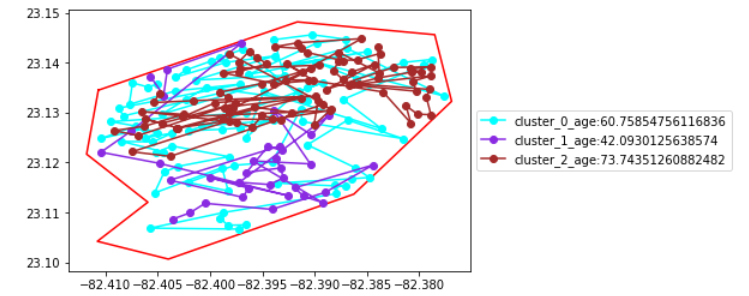
\includegraphics[width=\linewidth, height=3cm]{Images/Plaza.png}
		\caption{Plaza}
		\label{fig:Plaza}
	\end{subfigure}
	\begin{subfigure}[b]{0.49\linewidth}
		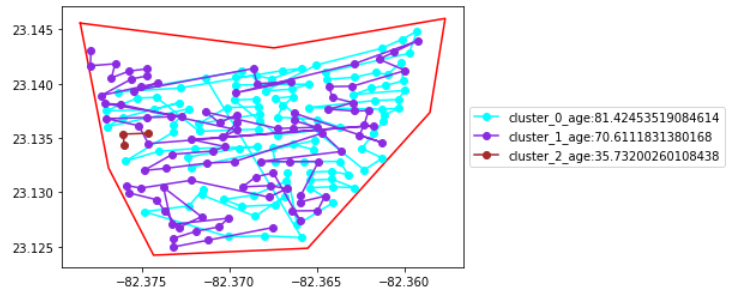
\includegraphics[width=\linewidth, height=3cm]{Images/CentroHabana.png}
		\caption{Centro Habana}
		\label{fig:CentroHab}
	\end{subfigure}
	\begin{subfigure}[b]{0.49\linewidth}
		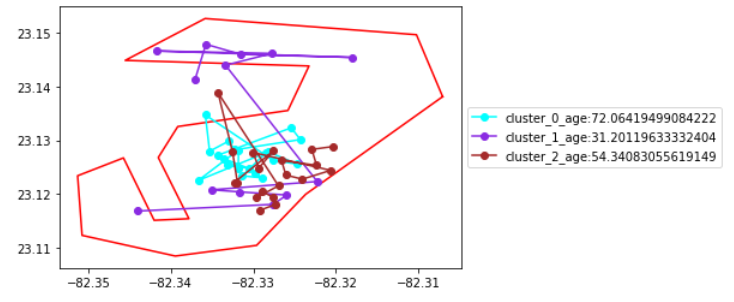
\includegraphics[width=\linewidth, height=3cm]{Images/Regla.png}
		\caption{Regla}
		\label{fig:Regla}
	\end{subfigure}
	\begin{subfigure}[b]{0.49\linewidth}
		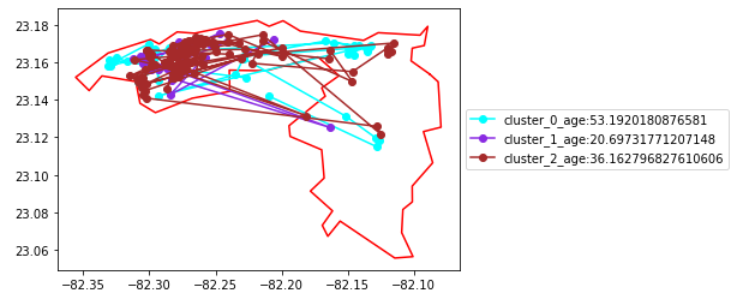
\includegraphics[width=\linewidth, height=3cm]{Images/HabEste.png}
		\caption{Habana del Este}
		\label{fig:HabEste}
	\end{subfigure}
	\begin{subfigure}[b]{0.49\linewidth}
		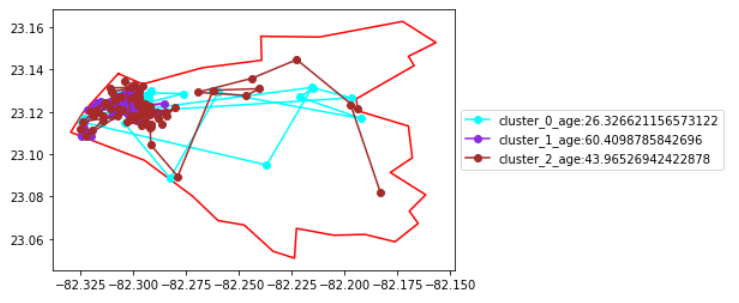
\includegraphics[width=\linewidth, height=3cm]{Images/Guanabacoa.png}
		\caption{Guanabacoa}
		\label{fig:Guanabacoa}
	\end{subfigure}
	\begin{subfigure}[b]{0.49\linewidth}
		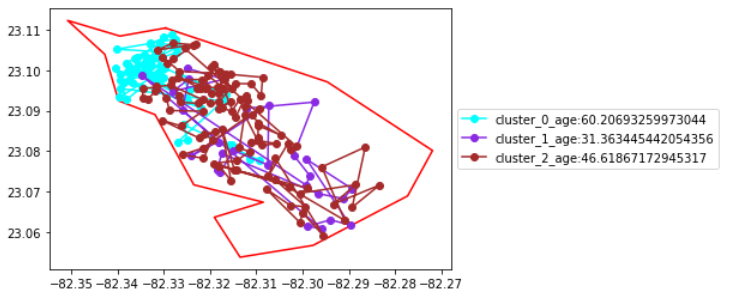
\includegraphics[width=\linewidth, height=3cm]{Images/SanMiguel.png}
		\caption{San Miguel del Padrón}
		\label{fig:SanMiguel}
	\end{subfigure}
	
	
	
	%\caption{Recorrido por el mapa}
	\label{fig:Resto de los municipios}
\end{figure}
\begin{figure}[h!]
	\centering
	\begin{subfigure}[b]{0.49\linewidth}
		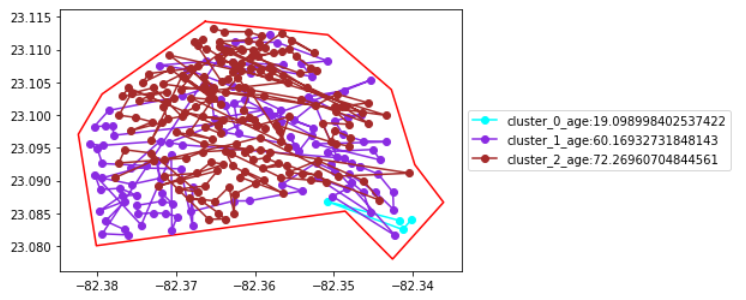
\includegraphics[width=\linewidth, height=3cm]{Images/10Otc.png}
		\caption{10 de Octubre}
		\label{fig:10Oct}
	\end{subfigure}
	\begin{subfigure}[b]{0.49\linewidth}
		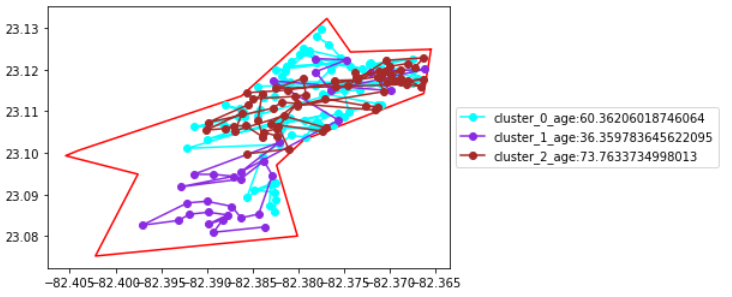
\includegraphics[width=\linewidth, height=3cm]{Images/Cerro.png}
		\caption{Cerro}
		\label{fig:Cerro}
	\end{subfigure}
	\begin{subfigure}[b]{0.49\linewidth}
		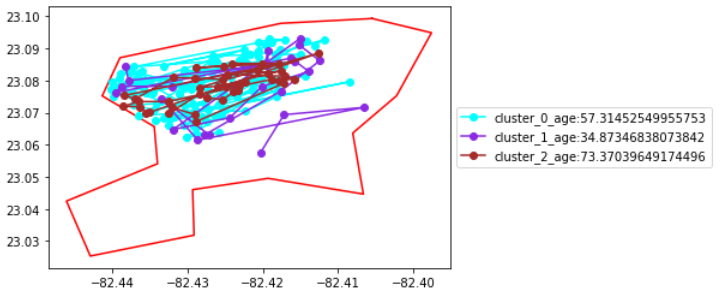
\includegraphics[width=\linewidth, height=3cm]{Images/Marianao.png}
		\caption{Marianao}
		\label{fig:Marianao}
	\end{subfigure}
	\begin{subfigure}[b]{0.49\linewidth}
		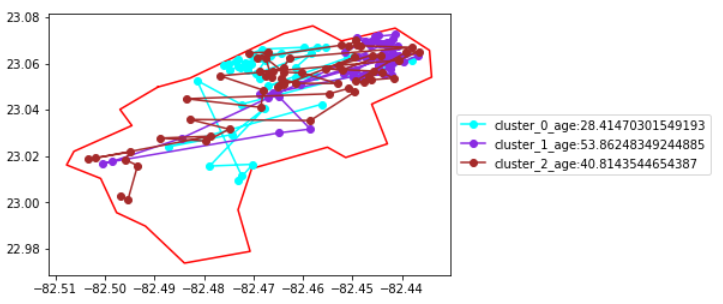
\includegraphics[width=\linewidth, height=3cm]{Images/LaLisa.png}
		\caption{La Lisa}
		\label{fig:Lisa}
	\end{subfigure}
	\begin{subfigure}[b]{0.49\linewidth}
		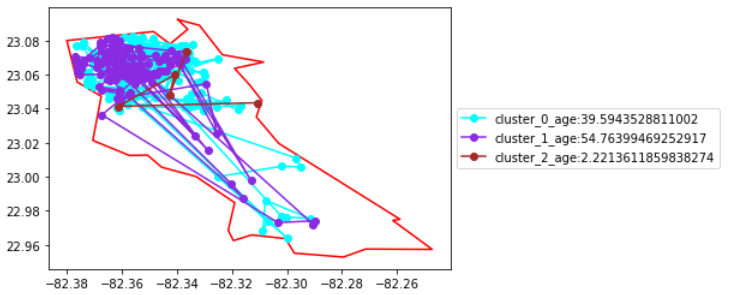
\includegraphics[width=\linewidth, height=3cm]{Images/ArroyoN.png}
		\caption{Arroyo Naranjo}
		\label{fig:Arroyo}
	\end{subfigure}
	\begin{subfigure}[b]{0.49\linewidth}
		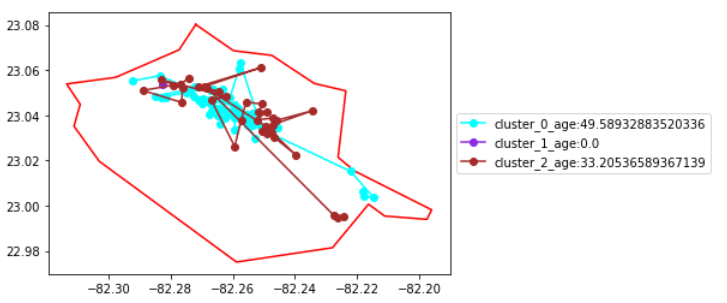
\includegraphics[width=\linewidth, height=3cm]{Images/Cotorro.png}
		\caption{Cotorro}
		\label{fig:Cotorro}
	\end{subfigure}
	
	%\caption{Recorrido por el mapa}
	\label{fig:RestoMunicipios1}
\end{figure}
\bibliographystyle{ieeetr}
\bibliography{Bibliography}


\end{document}